
% % Uncomment to build this alone without subfiles:
% % (also stuff at bottom)
% % \documentclass[draft]{scrbook} % visualise overfull hbox
% \documentclass{scrbook}
% % Koma script document options
\KOMAoption{paper}{a4}
\KOMAoption{fontsize}{11pt}
\KOMAoption{parskip}{half-} % paragraph spacing
% \KOMAoption{numbers}{enddot} % dot after section number
\KOMAoption{cleardoublepage}{plain} % include page numbers on blank pages
\KOMAoption{chapterprefix}{true} % 'Chapter' before number

% Packages
\usepackage{amsmath} % Gives \text command inside maths blocks
\usepackage{amssymb} % Various maths symbols
\usepackage{array} % Table formatting
\usepackage{bm} % Bold maths including Greek
\usepackage[format=plain]{caption} % Font sizing and alignment in captions
\usepackage{enumitem} % Allows numbering like 1.1 in ordered lists
% \usepackage{float} % Allows H placement of floats
\usepackage{graphicx}
\usepackage[hidelinks]{hyperref} % Hyperlinks without looking like it
% \usepackage{longtable} % Multi-page tables
% \usepackage{multicol} % For columns in text (not tables)
\usepackage{multirow} % For tables
\usepackage{neuralnetwork} % Neural net diagram
\usepackage{pdflscape} % Gives landscape environment
% \usepackage{scrlayer-scrpage} % To move page numbers
\usepackage{tabularx}
\usepackage{textcomp} % Added to fix \textasciiacute error on laptop
% \usepackage{tikz} % Diagrams (used for neural network example)
% \usepackage[pagenumberwidth=3em]{tocbasic}
% \usepackage{tocstyle} % ToC styling
\usepackage{upgreek} % Non-italic greek letters
\usepackage{xpatch} % Biblatex customisation

\usepackage[a4paper, inner=40mm, outer=15mm, top=30mm, bottom=30mm,footskip=15mm, headsep=15mm]{geometry}
% \usepackage[a4paper, inner=40mm, outer=30mm, top=50mm, bottom=50mm,footskip=20mm, headsep=20mm]{geometry} % footskip is space between footer (i.e. page number) and bottom of text
% min allowed is inner 40 mm, others 15 mm

\pagestyle{plain} % no header for front matter, overridden at end of front matter

% Caption setup
% \tablecaptionabove
\captionsetup[table]{labelsep=space}
% \captionsetup[table]{labelsep=space, skip=50pt, position=top}
\captionsetup[figure]{labelsep=space} % labelsep prevents dot followed by colon in captions

% Line spacing
\usepackage{setspace}
% \setstretch{1.4} % strangely this is > \onehalfspacing but < \doublespacing
\onehalfspacing
% \doublespacing

\raggedbottom % prevent huge spaces between paragraphs

% % % % % % % % % % % % % % % % % % % % % % % % %
% Font setup
% \usepackage{mathpazo} % Covers maths mode too
\usepackage[sc]{mathpazo} % Covers maths mode too, sc enables small caps
% \usepackage{palatino}
\usepackage[T1]{fontenc} % 8-bit font encoding
\addtokomafont{disposition}{\rmfamily} % Use serif throughout
% % % % % % % % % % % % % % % % % % % % % % % % %

% % % % % % % % % % % % % % % % % % % % % % % % %
% Section formatting setup
% \RedeclareSectionCommand[beforeskip=0pt]{chapter}
\RedeclareSectionCommand[beforeskip=0pt, innerskip=0pt]{chapter}
\RedeclareSectionCommand[beforeskip=10pt]{subsubsection}
\RedeclareSectionCommand[afterskip=1pt]{subsubsection}
% \setcounter{secnumdepth}{\subsubsectionnumdepth} % number up to subsubsections

% No dot after chapter number (https://tex.stackexchange.com/a/484727)
\renewcommand*{\chapterformat}{%
  \mbox{\chapappifchapterprefix{\nobreakspace}\thechapter
  \IfUsePrefixLine{}{\enskip}}%
}

% In the running header, separate chapter number and name with em dash
\renewcommand*{\chaptermarkformat}{%
\chapapp~\thechapter~---~}

% Create subsubsubsection below subsubsection but above paragraph, following https://tex.stackexchange.com/a/356574

\DeclareNewSectionCommand[
  style=section,
  counterwithin=subsubsection,
  afterskip=1pt,
  beforeskip=10pt,
  % afterskip=1.5ex plus .2ex,
  % beforeskip=3.25ex plus 1ex minus .2ex,
  % afterindent=false,
  level=\paragraphnumdepth,
  tocindent=10em,
  tocnumwidth=5em
]{subsubsubsection}
\setcounter{secnumdepth}{\subsubsubsectionnumdepth}
% \setcounter{tocdepth}{\subparagraphtocdepth}
\setcounter{tocdepth}{\subsubsubsectionnumdepth}

\RedeclareSectionCommands[
  level=\numexpr\subsubsubsectionnumdepth+1\relax,
  toclevel=\numexpr\subsubsubsectiontocdepth+1\relax,
  increaselevel,
]{paragraph,subparagraph}
\RedeclareSectionCommand[
  counterwithin=subsubsubsection,
  tocindent=12em,
  tocnumwidth=6em,
  beforeskip=10pt,
  afterskip=1pt, % line break after paragraph title
]{paragraph}
\RedeclareSectionCommand[
  tocindent=14em,
  tocnumwidth=7em,
  beforeskip=0pt
]{subparagraph}
% % % % % % % % % % % % % % % % % % % % % % % % %

% Autoref capitalisation
\def\chapterautorefname{Chapter}
\def\sectionautorefname{Section}
\def\subsectionautorefname{Section}
\def\subsubsectionautorefname{Section}

% % % % % % % % % % % % % % % % % % % % % % % % %
% Bibliography setup
\usepackage[backend=biber,
    % style=authoryear,
    style=authoryear-comp, % Don't repeat same author(s) in multiple citations
    giveninits=true,
    useprefix=true, % 'van der' etc.
    url=false,
    doi=false,
    isbn=false,
    eprint=false,
    uniquename=false, % Don't add initials in citation to disambiguate between authors with the same surname
    uniquelist=false, % Don't disambiguate in citation between different 'et al.' teams
    maxbibnames=10,
    minbibnames=10,
    maxcitenames=3,%  # 2,
    natbib, % Gives citep and citet commands
    labelalpha=true, % Use an 'alpha' label for each bib entry
    maxalphanames=1, % Use first author as the alpha label
    sorting=anyvt, % Sort by alpha (first author) then year
    block=par, % New line between 'blocks' of the bib entry
    dashed=false, % Reprint author list for each publication in bibliography
    sortcites=false % Show citations in the order supplied
]{biblatex}

% Citation/reference parameters
\renewcommand*{\nameyeardelim}{\addspace} % Space between author and year rather than comma
\renewcommand*{\finalnamedelim}{\addspace\&\addspace} % Ampersand rather than 'and'
\xpatchbibmacro{name:andothers}{{\finalandcomma}}{\addspace}{}{} % Space before 'et al.' rather than comma

% Citation-specific parameters
\DeclareCiteCommand{\blindcite}{\unspace}{}{}{\mancite} % Easy manual citations

% Reference-specific parameters
\AtEveryBibitem{\clearfield{title}} % Suppress title
\AtEveryBibitem{\clearfield{month}} % Suppress month
\DeclareNameAlias{author}{family-given} % Surname first for not just the first author
\DeclareNameAlias{editor}{family-given} % Same for editors
\renewbibmacro{in:}{} % Remove 'In:'
\DeclareFieldFormat{journaltitle}{#1} % Journal title in normal font rather than italics
\renewbibmacro*{volume+number+eid}{\printfield{volume}\printfield{number}\setunit{\addcomma\space}\printfield{eid}} % No dot after issue
\DeclareFieldFormat[article]{number}{\mkbibparens{#1}} % Volume in brackets
\DefineBibliographyStrings{english}{page = {}, pages = {}} % Suppress 'p.'/'pp.'
\renewbibmacro*{date+extradate}{\printtext{\printfield{year}\addcomma}} % Year not in brackets
\DeclareFieldFormat{pages}{\mkfirstpage[{\mkpageprefix[bookpagination]}]{#1}} % Only give starting page
\DeclareFieldFormat{url}{\url{#1}} % No 'URL' before URLs
% \renewcommand{\finentrypunct}{} % Remove final full stop
\renewcommand*{\newunitpunct}{\addcomma\space} % Commas between elements of bibitems

\DeclareBibliographyDriver{book}{%
  \printnames{author}%
  \space
  \printfield{year}%
  \newunit\newblock
  \printfield{booktitle}%
  \newunit
  , \printlist{publisher}%
\finentry}

\DeclareBibliographyDriver{inproceedings}{%
  \printnames{author}%
  \space
  \printfield{year}%
  \newunit\newblock
  \printfield{booktitle}%
  \newunit
  \printfield{volume}%
  \newunit
  \printfield{pages}%
\finentry}

\DeclareBibliographyDriver{incollection}{%
  \printnames{author}%
  \space
  \printfield{year}%
  \newunit\newblock
  \printfield{booktitle}%
  \newunit
  , ed. \printnames{editor},%
  \newunit\newblock
  \printlist{publisher}%
\finentry}

\DeclareBibliographyDriver{misc}{%
  \printnames{author}%
  \space
  \printfield{year}%
  \newunit\newblock
  \printfield{title}%
  \newunit
  \printfield{url}%
\finentry}

\addbibresource{refs.bib}
% % % % % % % % % % % % % % % % % % % % % % % % %

% Footnote spacing
% \deffootnote[1em]{1.5em}{1em}{\textsuperscript{\thefootnotemark~}}
\deffootnote[1em]{1em}{1em}{\textsuperscript{\thefootnotemark~}}

% Testing setting all penalties to zero
\binoppenalty=0
\brokenpenalty=0
\clubpenalty=0
\displaywidowpenalty=0
\exhyphenpenalty=0
\floatingpenalty=0
\hyphenpenalty=0
\interlinepenalty=0
% \linepenalty=0 % allowing this to be zero splits titles in a strange way
\postdisplaypenalty=0
\predisplaypenalty=0
\relpenalty=0
\widowpenalty=0

% Shorthands (non-Maths)
\newcommand{\lcdm}{$\Lambda$CDM}
\newcommand{\wcdm}{$w$CDM}
\newcommand{\Euclid}{\textit{Euclid}}
\newcommand{\Planck}{\textit{Planck}}
\newcommand{\Pcl}{Pseudo-$C_\ell$}
\newcommand{\pcl}{pseudo-$C_\ell$}
\newcommand{\ttp}{3$\times$2\,pt}

% Maths shorthands
\newcommand{\alm}{a_{\ell m}}
\newcommand{\Cl}{C_\ell}
\newcommand{\fsky}{f_\text{sky}}
\newcommand{\lmax}{\ell_\text{max}}
\newcommand{\lmin}{\ell_\text{min}}
\newcommand{\leff}{\ell_\text{eff}}
\newcommand{\tmin}{\theta_\text{min}}
\newcommand{\mathbfit}[1]{\bm{\mathit{#1}}}
\newcommand{\mathbfss}[1]{\bm{\mathsf{#1}}} % to match MNRAS \mathbfss
\renewcommand{\Re}{\operatorname{Re}}
\renewcommand{\Im}{\operatorname{Im}}

% ΛCDM parameters (maths mode)
\newcommand{\wo}{w_0}
\newcommand{\wa}{w_a}
\newcommand{\omm}{\Omega_\text{m}}
\newcommand{\omb}{\Omega_\text{b}}
\newcommand{\omc}{\Omega_\text{c}}
\newcommand{\sie}{\sigma_8}

% % Editing only
% \usepackage{xcolor}
% \newcommand{\todo}[1]{\textbf{{\color{red}{#1}}}}


% \usepackage{subfiles} % Best to do this last apparently

% \pagestyle{headings}
% \setcounter{chapter}{5} % deliberately 1 too low
% \begin{document}

% Uncomment to use subfiles:
% \documentclass[../Thesis.tex]{subfiles}
% \begin{document}

\chapter{Dependence of cosmological parameter constraints on angular binning of weak lensing two-point statistics}
\chaptermark{Dependence of parameter constraints on angular binning of two-point statistics} % short title for running header
\label{chap:binning}
\graphicspath{{../Figs/binning/}{Figs/binning/}}

\section{Introduction}

As introduced in \autoref{chap:est_like}, two-point statistics of weak lensing shear and galaxy number overdensity may be calculated in spherical harmonic space to estimate power spectra, or in real (also called configuration) space to estimate correlation functions. In either case, it is usually necessary to apply an angular binning in $\ell$ or $\theta$. For the power spectrum, this is not strictly necessary in principle, provided the effect of the survey mask is forward modelled rather than removed with a mixing matrix inversion (see the discussion of the \pcl{} method in \autoref{est_Sec:pcl}). However, a realistic \ttp{} analysis setup with 10 tomographic redshift bins and a scale cut of $\lmax = 5000$ would have a data vector with over a million elements if no angular binning was applied, which would be highly impractical. Furthermore, the smooth nature of weak lensing power spectra means that retaining a perfect angular resolution is probably unnecessary. For the correlation function, on the other hand, it is intrinsically necessary to bin in $\theta$, since galaxy pair separation is a continuous quantity sampled at particular points determined by the set of galaxies in the survey.

Varying numbers of angular bins have been used in recent weak lensing analyses. The Dark Energy Survey Year 3 analysis in \citet{DES2021} used 20 correlation function bins from 2.5 to 250 arcmin, while the KiDS-1000 analysis used 9 bins from 0.5 to 300 arcmin, and 8 bandpowers from $\ell = $ 100 to 1500 \citep{Joachimi2021, Heymans2021, Asgari2021}. The Hyper Suprime-Cam Year 1 \pcl{} analysis in \citet{Hikage2019} used 15 bandpowers from $\ell =$ 60 to 6500, though only 6 from $\ell =$ 300 to 1900 were retained in the cosmological analysis.

This chapter explores how many angular bins are necessary to retain a sufficient amount of constraining power in cosmological parameters. Specifically, it studies how the relative size of posterior uncertainties depends on the number of angular bins, both for the power spectrum and correlation function. Since angular binning will be essential in practice for upcoming Stage IV weak lensing surveys, it is vital to understand the relationship between this binning and cosmological parameter constraints in order to strike the optimal balance between computational viability and scientific value.

The main analysis of this chapter is contained within \autoref{bin_sec:main_analysis}, which studies how the size of parameter posterior uncertainties depends on the number of angular bins. In \autoref{bin_sec:additional_effects} a number of additional effects that may affect these results are examined. Conclusions are discussed in \autoref{bin_sec:conclusions}.

\section{Dependence of posterior uncertainties on number of angular bins}
\label{bin_sec:main_analysis}

This section contains the main analysis of the chapter. The method of measuring posterior uncertainties is described in \autoref{bin_sec:method}, while the observed dependence on the number of angular bins is described in \autoref{bin_sec:results}.

\subsection{Measurement of posterior uncertainties}
\label{bin_sec:method}

The posterior uncertainties in this section are measured directly from posterior distributions resulting from a full likelihood analysis. Later in the chapter, in \autoref{bin_sec:additional_effects}, methods will be described and used which approximate these results without the need for a full likelihood analysis.

The different elements of the likelihood analysis will now each be described.

\subsubsection{Modelling of two-point statistics}
\label{bin_sec:modelling}

\ttp{} power spectra were generated using \texttt{CosmoSIS} \citep{Zuntz2015}, covering a two-dimensional grid of values of $w_0$ and $w_a$, and one-dimensional grids of five other cosmological parameters ($\Omega_\text{m}$, $\Omega_\text{b}$, $\sigma_8$, $n_\text{s}$, $h$), with all other parameters held at fixed values in each case.
The pipeline is the same as described in \autoref{gl_Sec:fs_method_theory}, with five Gaussian redshift bins centred on $z =$ 0.65, 0.95, 1.25, 1.55, 1.85. Multipoles up to $\lmax = 5000$ were generated, but different scale cuts are explored in this chapter.
Power spectra were binned into bandpowers following Equation \eqref{cov_eqn:pbl}.

Angular-bin-averaged correlation functions for galaxy position $\xi_{NN}$, shear $\xi_\pm$, and their cross correlation $\xi_{NE}$, were calculated directly from the unbinned power spectra using the following relations:
\begin{align}
\xi_{NN} \left( \theta, \Delta \theta \right) &= \sum_\ell
\frac{2 \ell + 1}{4 \pi} C_\ell \,
\overline{d^\ell_{00}} \left( \theta, \Delta \theta \right);
% \end{equation}
% \begin{equation}
\\
\xi_\pm \left( \theta, \Delta \theta \right) &= \sum_\ell
\frac{2 \ell + 1}{4 \pi} C_\ell \,
\overline{d^\ell_{\pm22}} \left( \theta, \Delta \theta \right);
% \end{equation}
% \begin{equation}
\\
\xi_{NE} \left( \theta, \Delta \theta \right) &= \sum_\ell
\frac{2 \ell + 1}{4 \pi} C_\ell \,
\overline{d^\ell_{20}} \left( \theta, \Delta \theta \right),
\end{align}
where $\overline{d^\ell_{m' m}} \left( \theta, \Delta \theta \right)$ is the bin-averaged Wigner small-$d$ symbol. Following \citet{Fang2020b} and \citet{Stebbins1996}, the small-$d$ symbols may be written in terms of Legendre polynomials $P_\ell$, associated Legendre polynomials of order 2 $P_\ell^{m = 2}$,\footnote{Associated Legendre polynomials are defined as
\begin{equation}
P_\ell^m \left( x \right) =
\left( -1 \right)^m
\left( 1 - x^2 \right)^{m/2}
\frac{\text{d}^m}{\text{d}x^m}
P_\ell \left( x \right),
\end{equation}
such that
\begin{equation}
P_\ell \left( x \right) \equiv
P_\ell^{m = 0} \left( x \right).
\end{equation}} and Stebbins's $G$ symbol,
\begin{align}
d_{00}^\ell \left( \theta \right)
&= P_\ell \left( \cos \theta \right);
\\
% \end{equation}
% \begin{equation}
d_{\pm 2 2}^\ell \left( \theta \right)
&= \frac{2}{\ell^2 \left( \ell + 1 \right)^2}
\left[ G_{\ell, 2}^+ \left( \cos \theta \right)
\pm G_{\ell, 2}^- \left( \cos \theta \right) \right];
\\
%
% \end{equation}
% \begin{equation}
d_{2 0}^\ell \left( \theta \right)
&= \frac{1}{\ell \left( \ell + 1 \right)}
P_\ell^{m = 2} \left( \cos \theta \right),
\end{align}
which may be integrated analytically to obtain \citep{Friedrich2021, Fang2020b}
\begin{align}
\overline{P_\ell} \left( \theta, \Delta \theta \right) &=
\frac{1}{\cos \theta_2 - \cos \theta_1}
\frac{1}{2 \ell + 1}
\left[ P_{\ell + 1} \left( x \right) -
P_{\ell - 1} \left( x \right) \right]
_{x = \cos \theta_1}^{x = \cos \theta_2};
% {\left( 2 \ell + 1 \right)
% \left( \cos \theta_2 - \cos \theta_1 \right)};
\\[1em]
% % \end{equation}
% % \begin{equation}
% \overline{P_\ell} \left( \theta, \Delta \theta \right)
% &= \frac{\left[ P_{\ell + 1} \left( x \right) -
% P_{\ell - 1} \left( x \right) \right]
% _{x = \cos \theta_1}^{x = \cos \theta_2}}
% {\left( 2 \ell + 1 \right)
% \left( \cos \theta_2 - \cos \theta_1 \right)};
% % \end{equation}
% \\[1em]
%
% \begin{equation}
% \begin{aligned}[b]
\nonumber
\overline{G_{\ell, 2}^+ \pm G_{\ell, 2}^-}
\left( \theta, \Delta \theta \right) &=
\frac{1}{\cos \theta_2 - \cos \theta_1} \Bigg[
- \frac{\ell \left( \ell - 1 \right)}{2}
\left( \ell + \frac{2}{2 \ell + 1} \right)
P_{\ell - 1} \left( x \right)
\\ \nonumber
&~ - \frac{\ell \left( \ell - 1 \right) \left( 2 - \ell \right)}{2}
x P_\ell \left( x \right)
+ \frac{ \ell \left( \ell - 1 \right)}{2 \ell + 1}
P_{\ell + 1} \left( x \right)
\\ \nonumber
&~ + \left( 4 - \ell \right) \frac{d P_\ell \left( x \right)}{dx}
+ \left( \ell + 2 \right)
\left( x \frac{d P_{\ell - 1} \left( x \right)}{dx}
- P_{\ell - 1} \left( x \right) \right)
\\
&~ \pm 2 \left( \ell - 1 \right)
\left( x \frac{dP_\ell \left( x \right)}{dx}
- P_\ell \left( x \right) \right)
\mp 2 \left( \ell + 2 \right)
\frac{dP_{\ell - 1}\left( x \right)}{dx}
\Bigg]_{x = \cos \theta_1}^{x = \cos \theta_2};
\\[1em]
% \end{aligned}
% \end{equation}
% \begin{equation}
% \begin{aligned}[b]
\nonumber
\overline{P_\ell^{m = 2}} \left( \theta, \Delta \theta \right)
&= \frac{1}{\cos \theta_2 - \cos \theta_1} \Bigg[
\left( \ell + \frac{2}{2 \ell + 1} \right) P_{\ell - 1} \left( x \right)
+ \left( 2 - \ell \right) x P_\ell \left( x \right)
\\ &\qquad\qquad\qquad\qquad\qquad\qquad\qquad\qquad
- \frac{2}{2 \ell + 1} P_{\ell + 1} \left( x \right)
\Bigg]_{x = \cos \theta_1}^{x = \cos \theta_2},
% \end{aligned}
\end{align}
where $\theta_1 = \theta$ and $\theta_2 = \theta + \Delta \theta$. The only symbols necessary to evaluate these equations are the Legendre polynomials and their derivatives, which are evaluated up to a required $\ell_\text{max}$ using the \texttt{SciPy} Python library \citep{Virtanen2020}. These transforms assume a uniform distribution of galaxies, which corresponds to a distribution of galaxy pairs proportional to $\sin{\theta}$ \citep{Friedrich2021}. The angular bins are logarithmically spaced for both the power spectra and correlation functions.

Noise was added to the power spectra prior to binning, following Equations \eqref{gl_Eqn:nl_start}--\eqref{gl_Eqn:nl_end}, with a number density of $6 / \text{arcmin}^2$ in each of five redshift bins, and an intrinsic shape dispersion of $\sigma_\epsilon = 0.3$ per component. For the correlation functions, noise only contributes via the covariance, which is described in \autoref{bin_sec:likelihood} below.

\subsubsection{Likelihood and covariance}
\label{bin_sec:likelihood}

A Gaussian likelihood was used for both the power spectra and correlation functions. This was shown to be sufficiently accurate for power spectra in \autoref{chap:gauss_like}. It can also be expected to be sufficiently accurate for correlation functions, since they are simply linear transformations of power spectra. To remove any unwanted randomness from the size of the posterior uncertainties, no observed realisation was simulated and instead the model data vector was used at the fiducial parameter values.

The covariance of the unbinned power spectrum was calculated assuming Gaussian fields, following Equation \eqref{gl_Eqn:cov_g}. This was then transformed linearly to obtain both the covariance of the binned power spectrum and the binned correlation function, using the general rule that for any data vector $\bm{x}$ having covariance matrix $\bm{\Sigma}$, the covariance of $\mathbfss{M} \bm{x}$, where $\mathbfss{M}$ is the matrix representing some general linear transformation, is given by
\begin{equation}
\text{Cov} \left( \mathbfss{M} \bm{x} \right)
% = \bm{\Sigma} \mathbfss{M} \bm{\Sigma}^\intercal.
= \mathbfss{M} \bm{\Sigma} \mathbfss{M}^\intercal.
\end{equation}

For the power spectrum, noise was included in the unbinned $\Cl$s used to calculate the covariance, as described above in \autoref{bin_sec:modelling}. For the correlation function, noise-free $\Cl$s were used, and a noise contribution to the diagonal of the covariance was added using the following expressions \citep{Schneider2002, Joachimi2008, Heymans2013, Troxel2018}
\begin{align}
% +/-, +/-
\text{Cov}_\text{Noise} \left( \xi^{ij}_{NN} \left( \theta_1 \right),
\xi^{kl}_{NN} \left( \theta_2 \right) \right)
&= \frac{1} {N_\text{p}^{ij} \left( \theta_1, \Delta \theta_1  \right)}
\delta_{\theta_1 \theta_2}
\left( \delta_{ik} \delta_{jl} + \delta_{il} \delta_{jk} \right);
\label{bin_Eq:noise_cov_start}
% \end{equation}
% \begin{equation}
\\[1em]
%
% +, +
\text{Cov}_\text{Noise} \left( \xi^{ij}_+ \left( \theta_1 \right),
\xi^{kl}_+ \left( \theta_2 \right) \right)
&= \frac{\left( \sigma_\epsilon^i \sigma_\epsilon^j \right)^2}
{N_\text{p}^{ij} \left( \theta_1, \Delta \theta_1  \right)}
\delta_{\theta_1 \theta_2}
\left( \delta_{ik} \delta_{jl} + \delta_{il} \delta_{jk} \right);
% \end{equation}
% \begin{equation}
\\[1em]
%
% -, -
\text{Cov}_\text{Noise} \left( \xi^{ij}_- \left( \theta_1 \right),
\xi^{kl}_- \left( \theta_2 \right) \right)
&= \frac{\left( \sigma_\epsilon^i \sigma_\epsilon^j \right)^2}
{N_\text{p}^{ij} \left( \theta_1, \Delta \theta_1  \right)}
\delta_{\theta_1 \theta_2}
\left( \delta_{ik} \delta_{jl} + \delta_{il} \delta_{jk} \right);
% \end{equation}
% \begin{equation}
\\[1em]
%
% NE, NE
\text{Cov}_\text{Noise} \left( \xi^{ij}_{NE} \left( \theta_1 \right),
\xi^{kl}_{NE} \left( \theta_2 \right) \right)
&= \frac{\left( \sigma_\epsilon^i \sigma_\epsilon^j \right)^2}
{N_\text{p}^{ij} \left( \theta_1, \Delta \theta_1  \right)}
\delta_{\theta_1 \theta_2}
\delta_{ik} \delta_{jl}.
\label{bin_Eq:noise_cov_end}
\end{align}

In Equations \eqref{bin_Eq:noise_cov_start}--\eqref{bin_Eq:noise_cov_end}, $i$--$l$ represent redshift bins, $\sigma_\epsilon^i$ and $\sigma_\epsilon^j$ are the intrinsic shape dispersion per component in each redshift bin, and $N_\text{p}$ is the number of galaxy pairs in a particular angular bin, given by \citep{Friedrich2021}
\begin{equation}
N_\text{p}^{ij} = \frac{1}{2} \, A_\text{survey} \, A_\text{bin} \, N_i \, N_j,
\end{equation}
where $A_\text{survey}$ is the survey area in steradians, $N_i$ and $N_j$ are the galaxy number densities in bins $i$ and $j$, and $A_\text{bin}$ is the angular bin area given by
\begin{equation}
A_\text{bin} = 2 \pi \left[
\cos{\left( \theta \right)}
-
\cos{\left( \theta + \Delta \theta \right)}
\right].
\end{equation}

\subsubsection{Cut-sky treatment}

\begin{figure}[t]
\centering
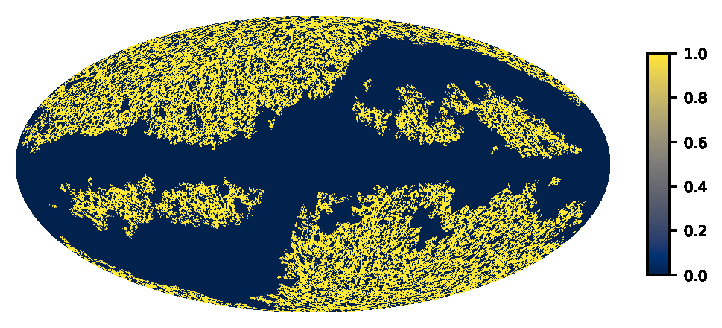
\includegraphics[width=.7\textwidth]{mask}
\caption{The Stage-IV-like mask describing a fictitious satellite-based survey used for the cut-sky results in this chapter.}
\label{bin_Fig:mask}
\end{figure}

For the cut-sky results, a Stage-IV-like mask describing a fictitious satellite-based survey was used. This was obtained by transforming the WMAP temperature mask used in \autoref{chap:exact_like} \citep{Bennett2013}, to excise the ecliptic plane in addition to the galactic plane. Additional point-source holes were added until a desired sky coverage of $\fsky = 0.3$ was achieved. The centre of each hole was chosen by selecting pixels at random. The immediate neighbouring pixels were also excised, after which a recursive probabilistic method was used, with a 50\% chance of the next neighbouring pixels being removed, and so on up to a maximum hole radius of 6 pixels. The final mask is shown in \autoref{bin_Fig:mask}.

The impact of the sky cut on observed power spectra was modelled using a mixing matrix obtained using \texttt{NaMaster} \citep{Alonso2019}. A cut-sky power spectrum covariance was obtained using the improved narrow kernel approximation \citep{Nicola2021} method described in \autoref{chap:cov}. The sky cut does not affect the expected value of the correlation function, but does affect its covariance. This is modelled by applying a factor of $1 / \fsky$ to the full-sky covariance matrix. Although this is presumably an approximation, it is standard practice for the cut-sky correlation function, used for example in the DES Year 3 covariance described in \citet{Friedrich2021}. It was shown in \citet{Cabre2007} that this `$\fsky$ approximation' is a good approximation to the simulated cut-sky correlation function covariance, which is not the case for the power spectrum. Nevertheless, in \autoref{bin_sec:fsky} it is shown that the use of this approximation for the power spectrum does not significantly affect the dependence of posterior uncertainties on the number of angular bins. Therefore, it can be expected to be a sufficiently accurate approximation for the correlation function in this chapter.

\subsection{Posterior uncertainty as a function of number of angular bins}
\label{bin_sec:results}

\begin{figure}[t]
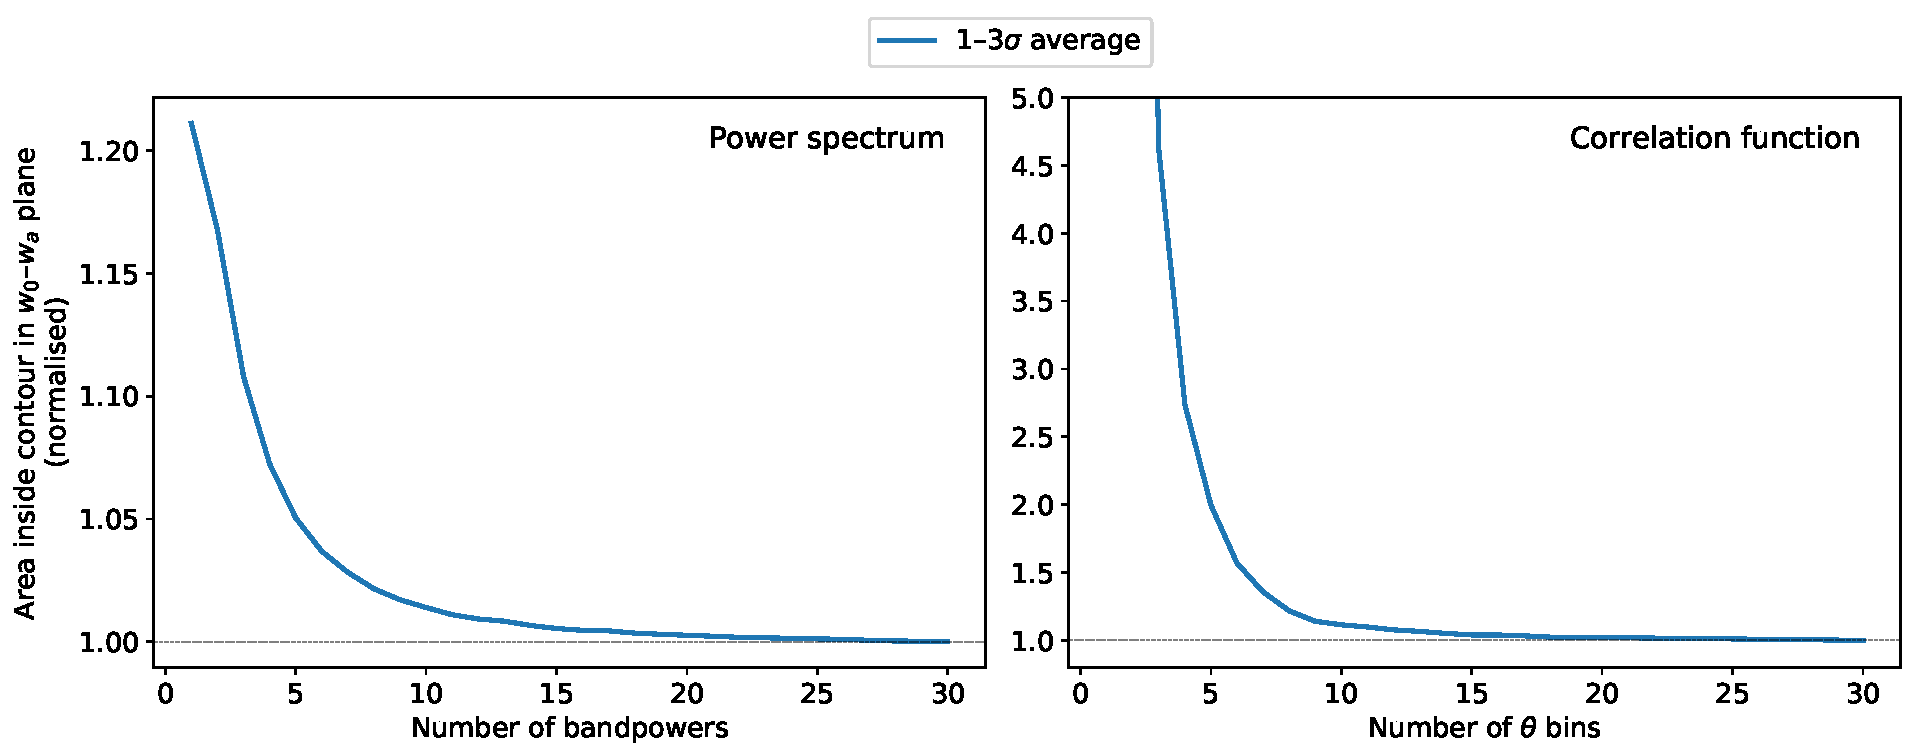
\includegraphics[width=\textwidth]{area_vs_nbin_fs}
\caption{Dependence of posterior uncertainties in a joint full-sky analysis of $w_0$ and $w_a$ on the number of angular bins for the power spectrum (left) and correlation function (right). Each line is averaged over 100 contours linearly spaced from $1\sigma$ to $3\sigma$ and normalised to be equal to 1 at its minimum, as described in the first paragraph of \autoref{bin_sec:results}.}
\label{bin_Fig:area_vs_nbin_fs}
\end{figure}

The dependence of posterior uncertainties in a joint full-sky analysis of $w_0$ and $w_a$ on the number of angular bins is shown for the power spectrum and correlation function in \autoref{bin_Fig:area_vs_nbin_fs}.
% Each line is averaged over 100 contours linearly spaced from $1\sigma$ to $3\sigma$ and normalised to be equal to 1 at its minimum.
Each line is calculated by forming the joint posterior distribution of $w_0$ and $w_a$, drawing 100 credible regions linearly spaced from $1\sigma$ to $3\sigma$ (following the definitions of credible regions and sigma notation described in \autoref{est_Sec:credible_regions_sigma_notation}), measuring the area of every credible region as a function of the number of angular bins, normalising each curve to be equal to 1 at its minimum, and finally averaging over all 100 regions. This technique removes most of the noise that results from the finite resolution of the posterior grids.

\begin{figure}[t]
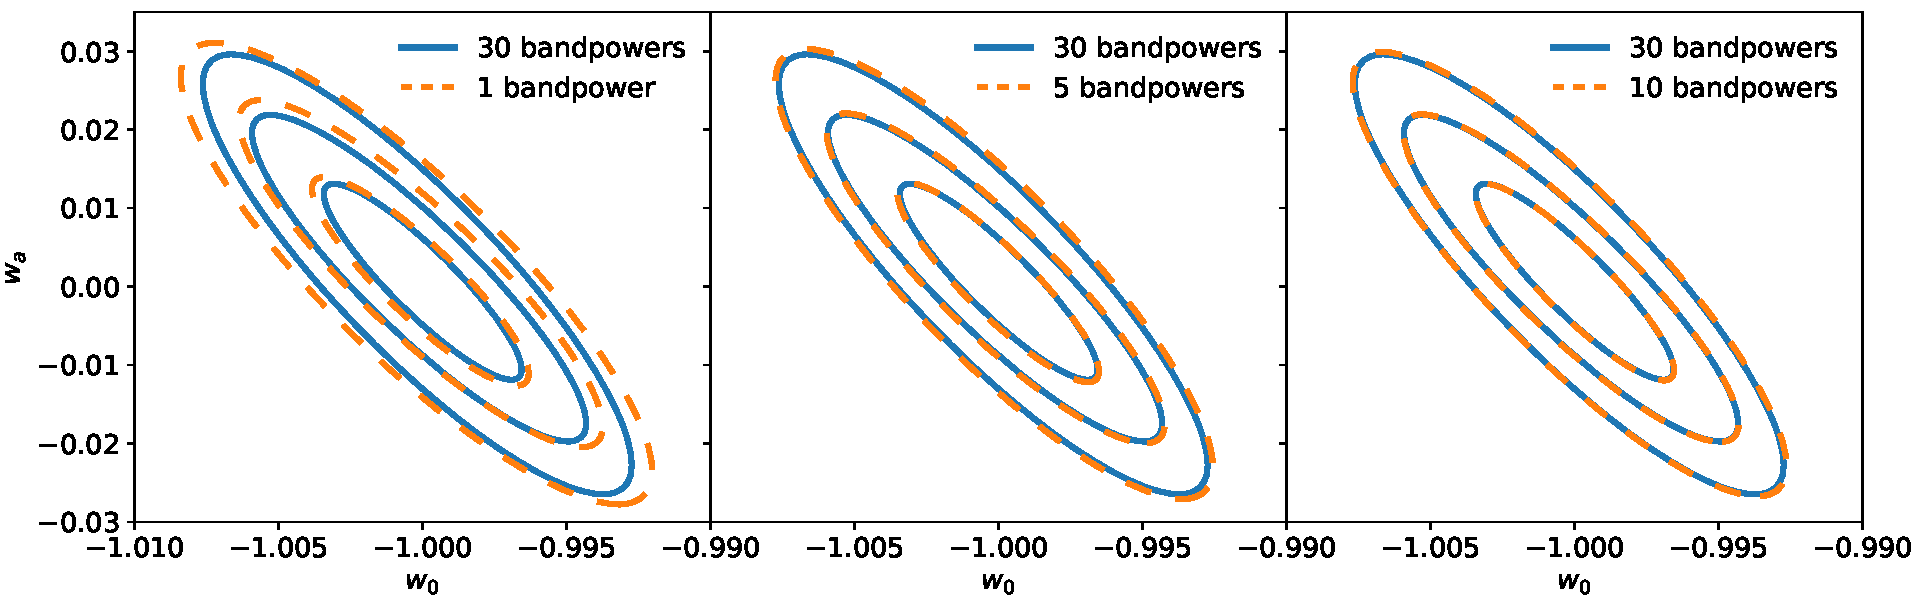
\includegraphics[width=\textwidth]{posts_w0wa_cl}
\caption{1--3$\sigma$ posterior contours from the full-sky power spectrum with different numbers of bandpowers used in the likelihood analysis.}
\label{bin_Fig:posts_w0wa_cl}
\end{figure}

\begin{figure}[t]
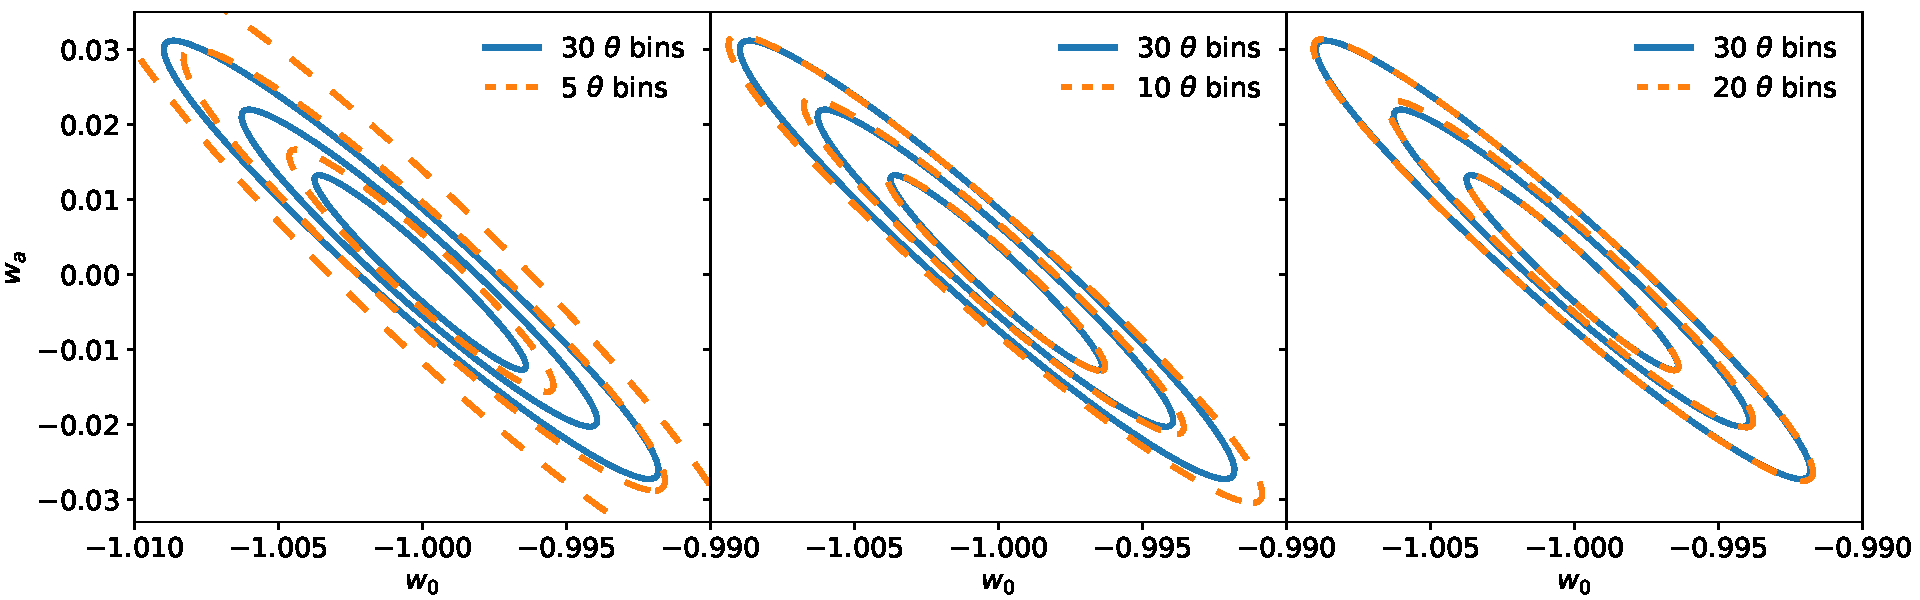
\includegraphics[width=\textwidth]{posts_w0wa_cf}
\caption{As \autoref{bin_Fig:posts_w0wa_cl} but for the correlation function. 1--3$\sigma$ posterior contours from the full-sky correlation function with different numbers of angular bins used in the likelihood analysis.}
\label{bin_Fig:posts_w0wa_cf}
\end{figure}

\begin{figure}[t]
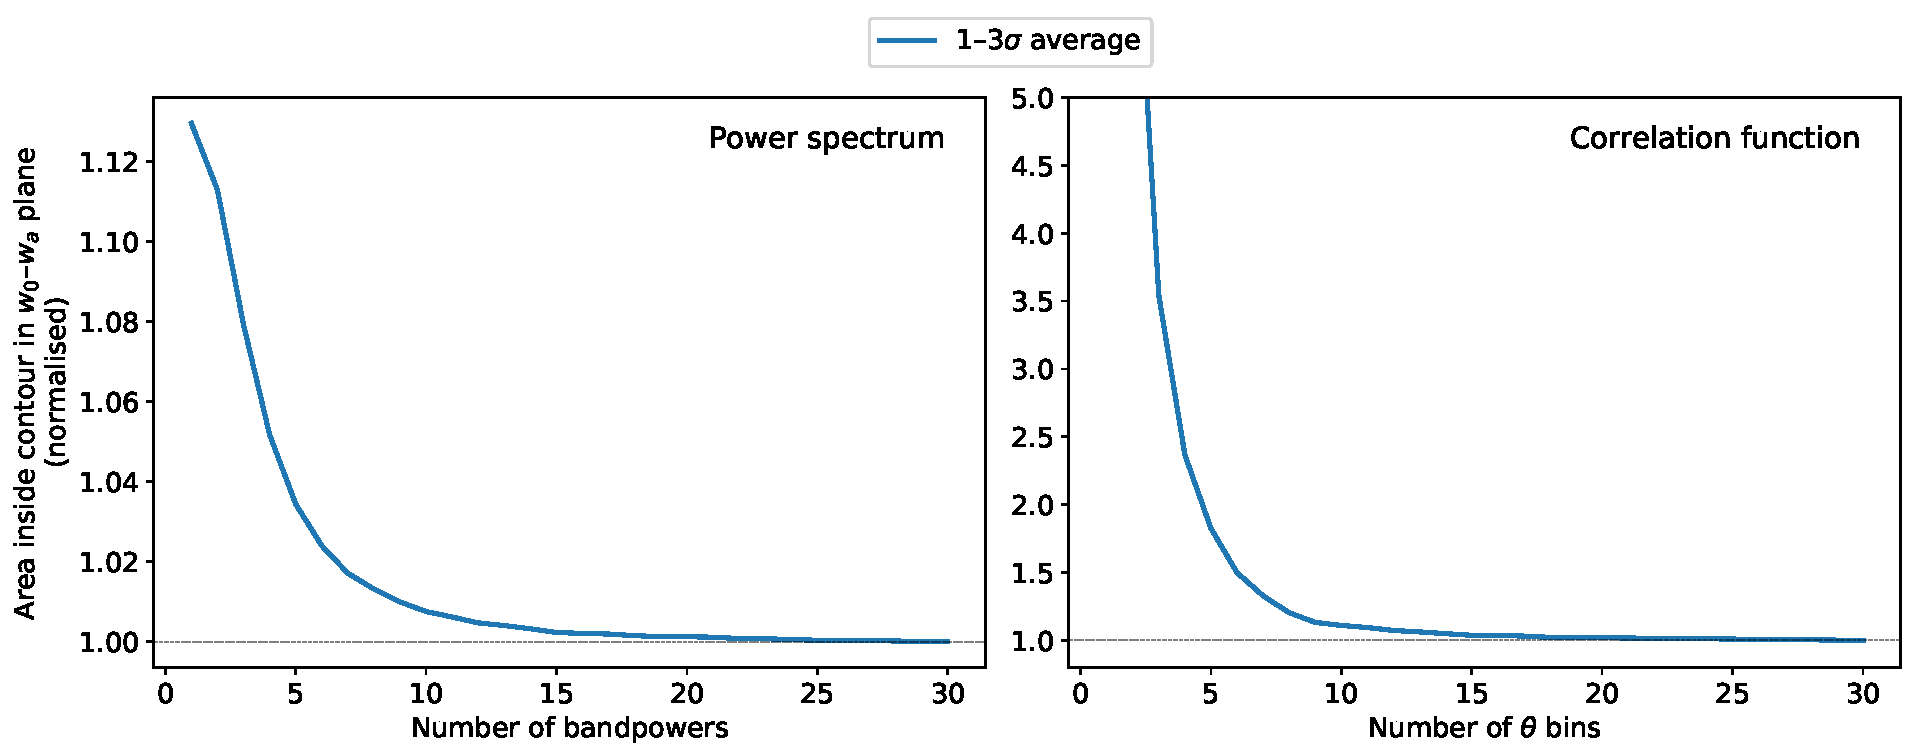
\includegraphics[width=\textwidth]{area_vs_nbin_ma}
\caption{As \autoref{bin_Fig:area_vs_nbin_fs} but for a cut-sky analysis. Dependence of posterior uncertainties in a joint cut-sky analysis of $w_0$ and $w_a$ on the number of angular bins for the power spectrum (left) and correlation function (right). Each line is averaged over 100 contours linearly spaced from $1\sigma$ to $3\sigma$ and normalised to be equal to 1 at its minimum, as described in the first paragraph of \autoref{bin_sec:results}.}
\label{bin_Fig:area_vs_nbin_ma}
\end{figure}

\begin{figure}[t!]
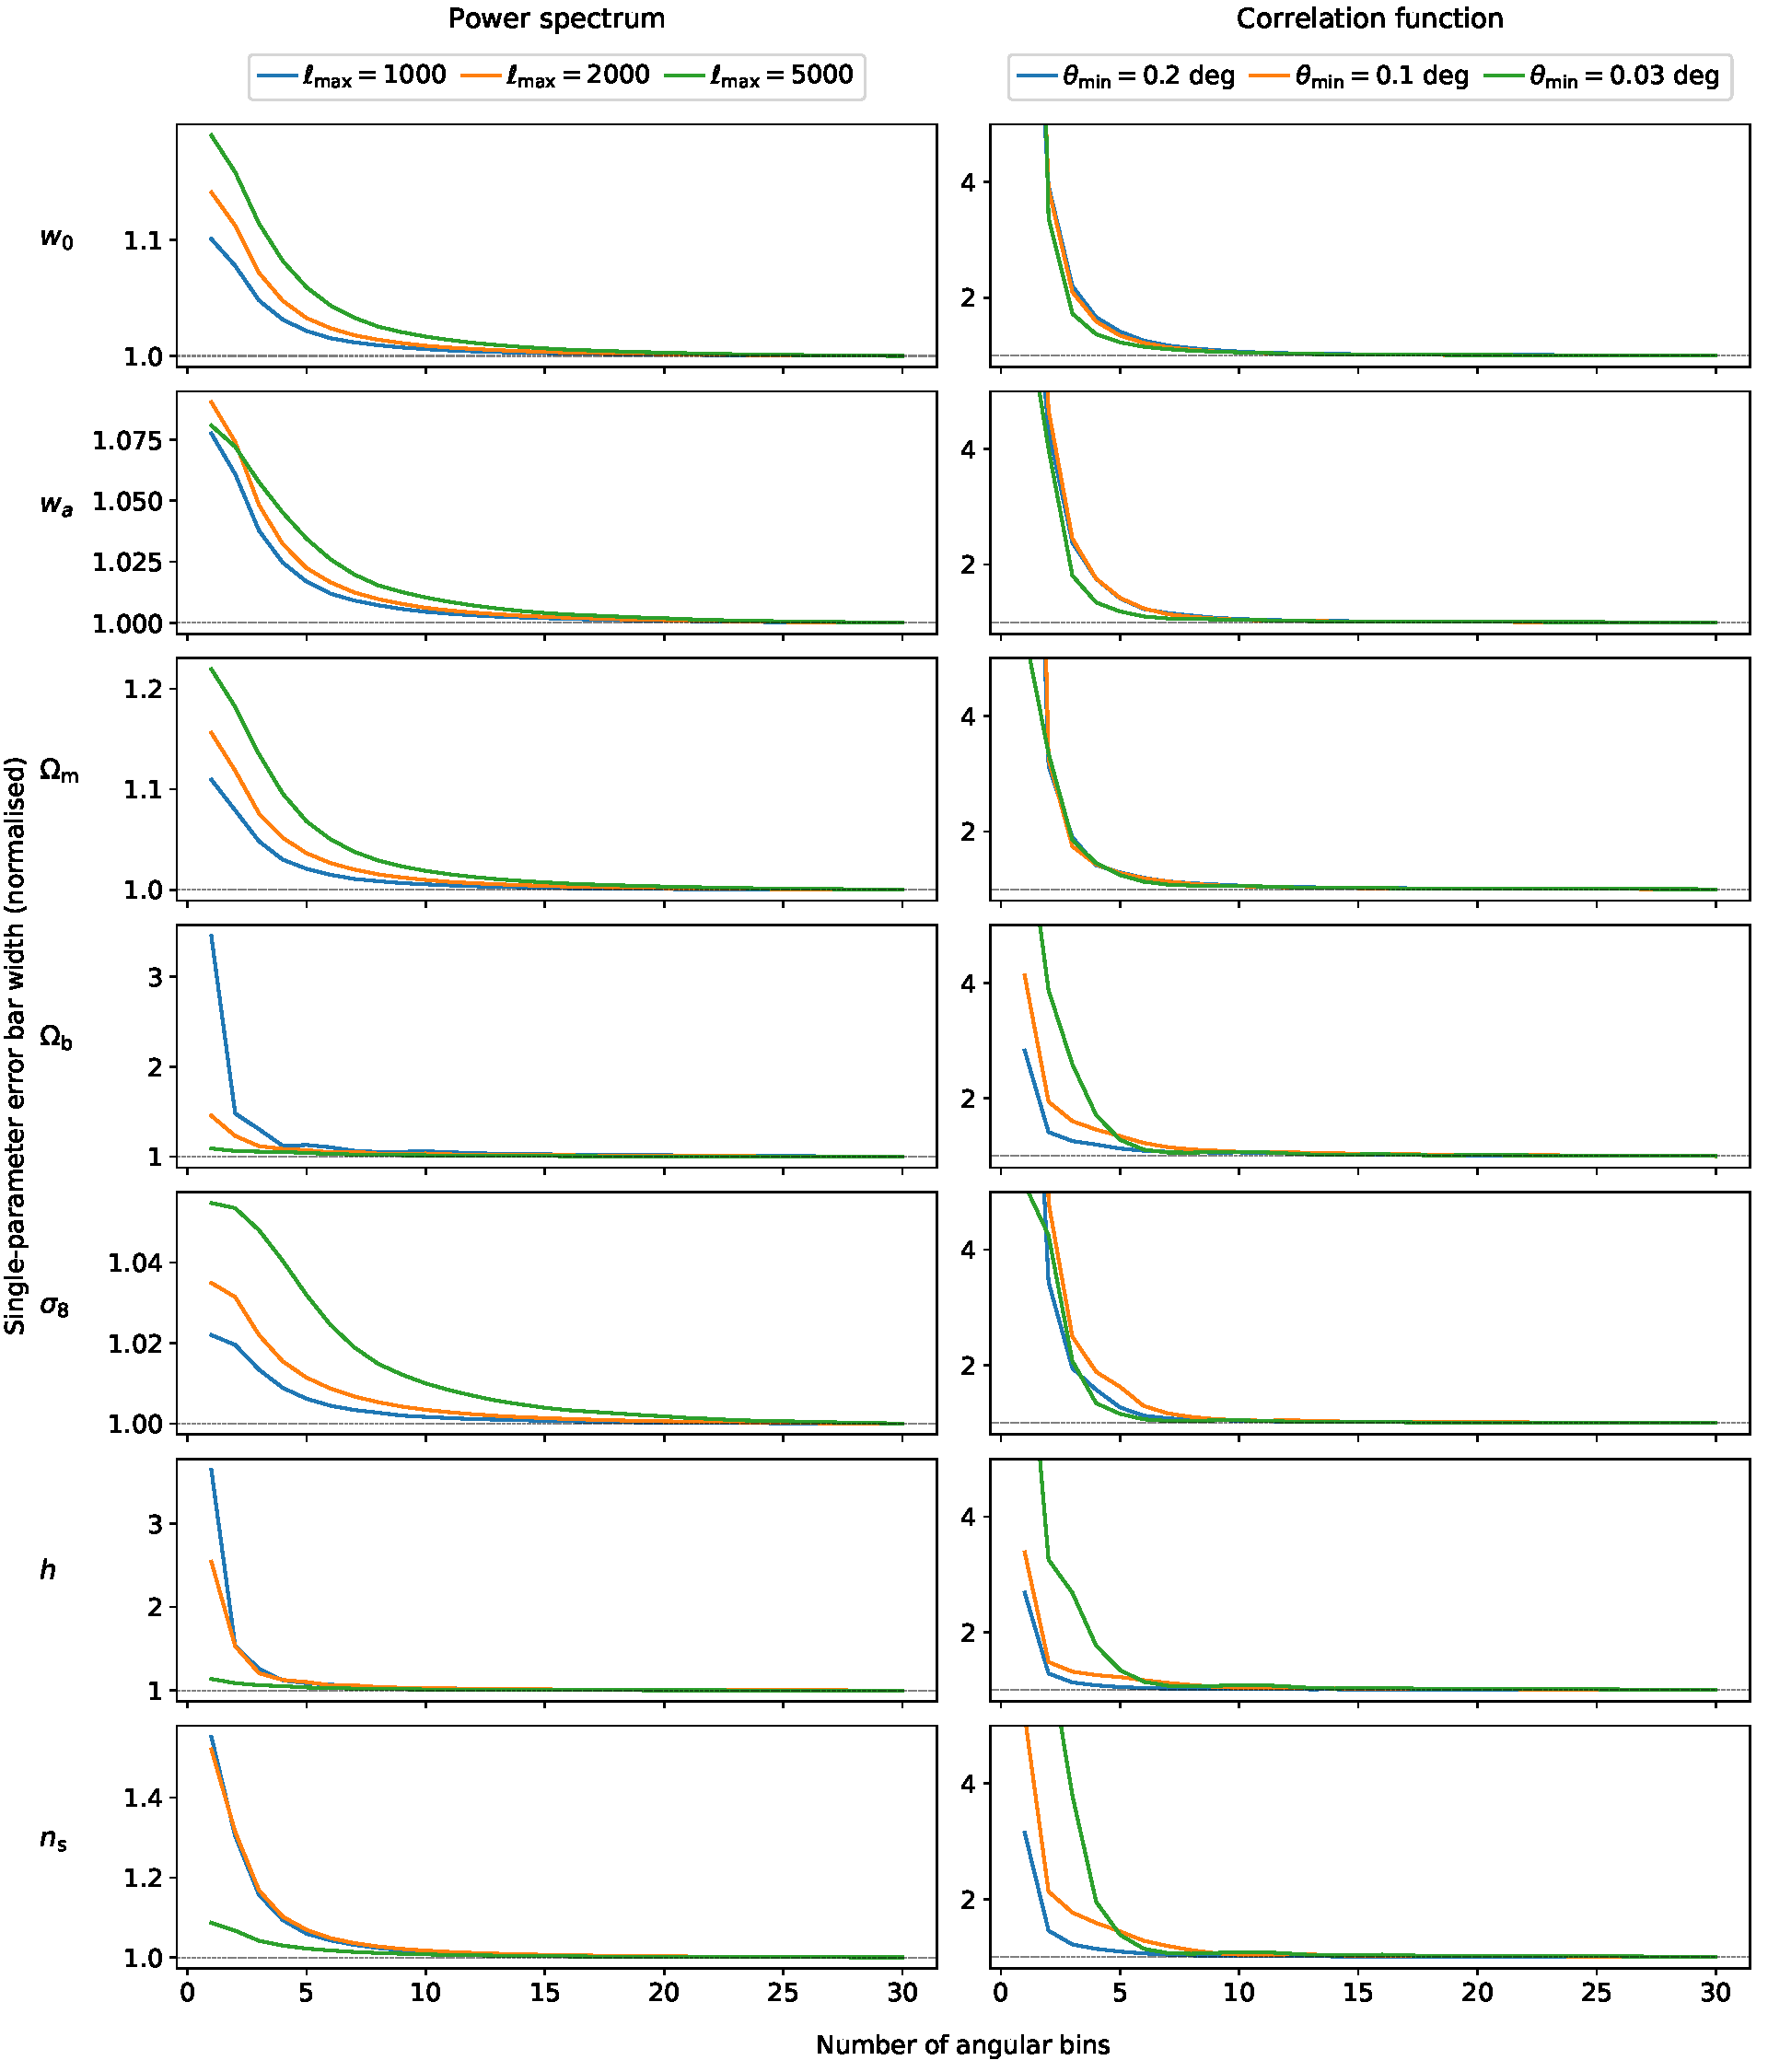
\includegraphics[width=\textwidth]{width_vs_nbin}
\caption{As \autoref{bin_Fig:area_vs_nbin_fs} but for a single parameter at a time. Dependence of posterior uncertainties in a single-parameter analysis on the number of angular bins for the power spectrum (left) and correlation function (right). Each line is averaged over 100 contours linearly spaced from $1\sigma$ to $3\sigma$ and normalised to be equal to 1 at its minimum, as described in the first paragraph of \autoref{bin_sec:results}. Each parameter is constrained independently, with all other parameters held fixed. The results for different scale cuts are shown in different colours.}
\label{bin_Fig:width_vs_nbin}
\end{figure}

Both lines in \autoref{bin_Fig:area_vs_nbin_fs} are mostly flat above around 10 angular bins, and converge to a minimum by around 20--25 bins. Below 10 bins, there is a sharp increase in contour area. For the power spectrum, however, this only reaches a maximum of around 20 per cent higher than the minimum area, even for a single bandpower. In contrast, the contour area for the correlation function diverges sharply at around 5 bins. This difference in behaviour is explored in \autoref{bin_sec:low_nbin}.

To further illustrate the dependence shown in \autoref{bin_Fig:area_vs_nbin_fs}, posterior distributions with different numbers of angular bins are shown in \autoref{bin_Fig:posts_w0wa_cl} for the full-sky power spectrum and in \autoref{bin_Fig:posts_w0wa_cf} for the full-sky correlation function. It can be seen in the left panel of \autoref{bin_Fig:posts_w0wa_cl} that the single-bandpower posterior distribution is only slightly larger than the equivalent result with 30 bandpowers. The correlation function posteriors in \autoref{bin_Fig:posts_w0wa_cf} show more degradation as the number of bins is decreased, as mentioned above.

\autoref{bin_Fig:area_vs_nbin_ma} shows the same dependence on the number of angular bins, but this time for a cut-sky analysis. The results are very similar to the full-sky results in \autoref{bin_Fig:area_vs_nbin_fs}. For this reason, the remainder of this chapter considers only a full-sky setup, but the conclusions should be applicable to a cut-sky analysis as well.

Additional cosmological parameters are investigated in \autoref{bin_Fig:width_vs_nbin}. These are chosen to be the parameters included in the \Euclid{} forecast paper \citep{Blanchard2020}: $w_0$, $w_a$, $\Omega_\text{m}$, $\Omega_\text{b}$, $\sigma_8$, $n_\text{s}$, $h$. These parameters are described in \autoref{chap:cosmo}. Each parameter is shown for three different scale cuts. For the power spectrum, the maximum multipole $\lmax$ is varied from the baseline value of $\lmax = 2000$ to a more conservative $\lmax = 1000$ and a more optimistic $\lmax = 5000$. For the correlation function, the respective equivalent minimum separation $\tmin$ values are $\tmin =$ 0.1\,deg, $\tmin =$ 0.2\,deg, and $\tmin =$ 0.03\,deg. While the different parameters behave broadly similarly, there are some differences. For example, while some parameters such as $w_0$ only exhibit a 10--20 per cent degradation at low numbers of bandpowers, others such as $\omb$ exhibit as much as 300 per cent degradation, perhaps because constraining such parameters requires sufficient angular resolution to resolve the shape of the power spectrum and not just its amplitude.

\begin{figure}[t]
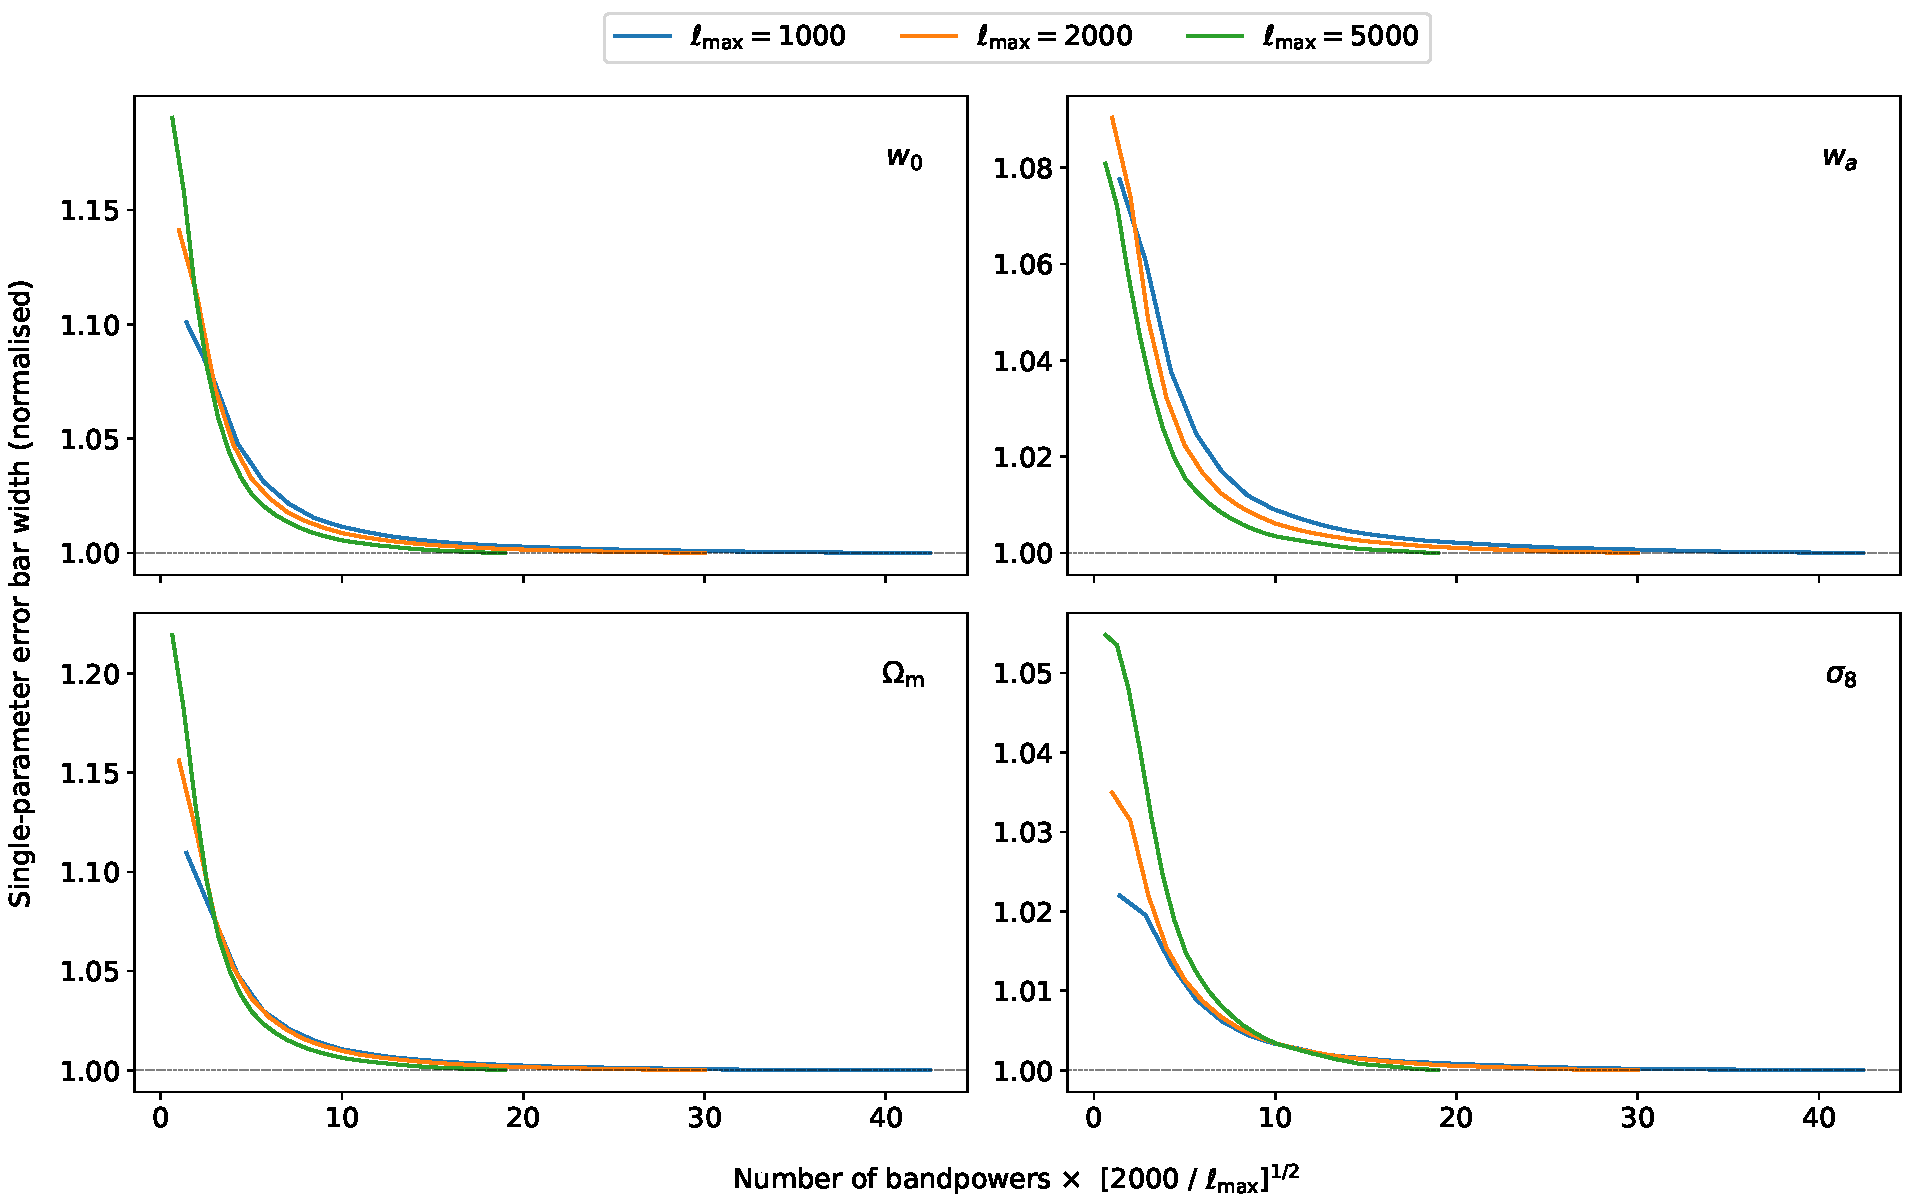
\includegraphics[width=\textwidth]{sqrt_lmax}
\caption{Dependence on the number of bandpowers for the full-sky power spectrum, for four parameters exhibiting a particular property: the number of bandpowers required for a particular level of degradation for different $\lmax$ values approximately scales as $\sqrt{\lmax}$.}
\label{bin_Fig:sqrt_lmax}
\end{figure}

Ideally it would be possible to unify the results with different scale cuts in \autoref{bin_Fig:width_vs_nbin} into a dependence on a single measure, such as the logarithmic angular bin size. However, the different parameters behave differently as $\lmax$ and $\tmin$ are varied, so this is not possible in practice. However, a certain subset of the parameters do exhibit such a convenient property for the power spectrum: it is shown in \autoref{bin_Fig:sqrt_lmax} that for four parameters---$\wo$, $\wa$, $\omm$ and $\sie$---the number of bandpowers required for a given $\lmax$ value scales approximately as $\sqrt{\lmax}$. The reason for this particular dependence is not clear, but it is perhaps not a coincidence that these parameters are those which depend most on the amplitude of weak lensing power spectra and least on their shape. For this reason, these parameters are also the most strongly correlated in a \Euclid{}-like analysis \citep{Blanchard2020}.

\section{Exploration of additional effects}
\label{bin_sec:additional_effects}

In this section, three different effects which may affect the required number of angular bins are explored. \autoref{bin_sec:fsky} investigates the impact of the $\fsky$ approximation in the power spectrum covariance. \autoref{bin_sec:low_nbin} explores why the power spectrum and correlation function exhibit such different behaviour for low numbers of angular bins, while \autoref{bin_Sec:noise} studies the impact of noise.

\subsection{Impact of \texorpdfstring{$\fsky$}{fsky} approximation}
\label{bin_sec:fsky}

\begin{figure}[t]
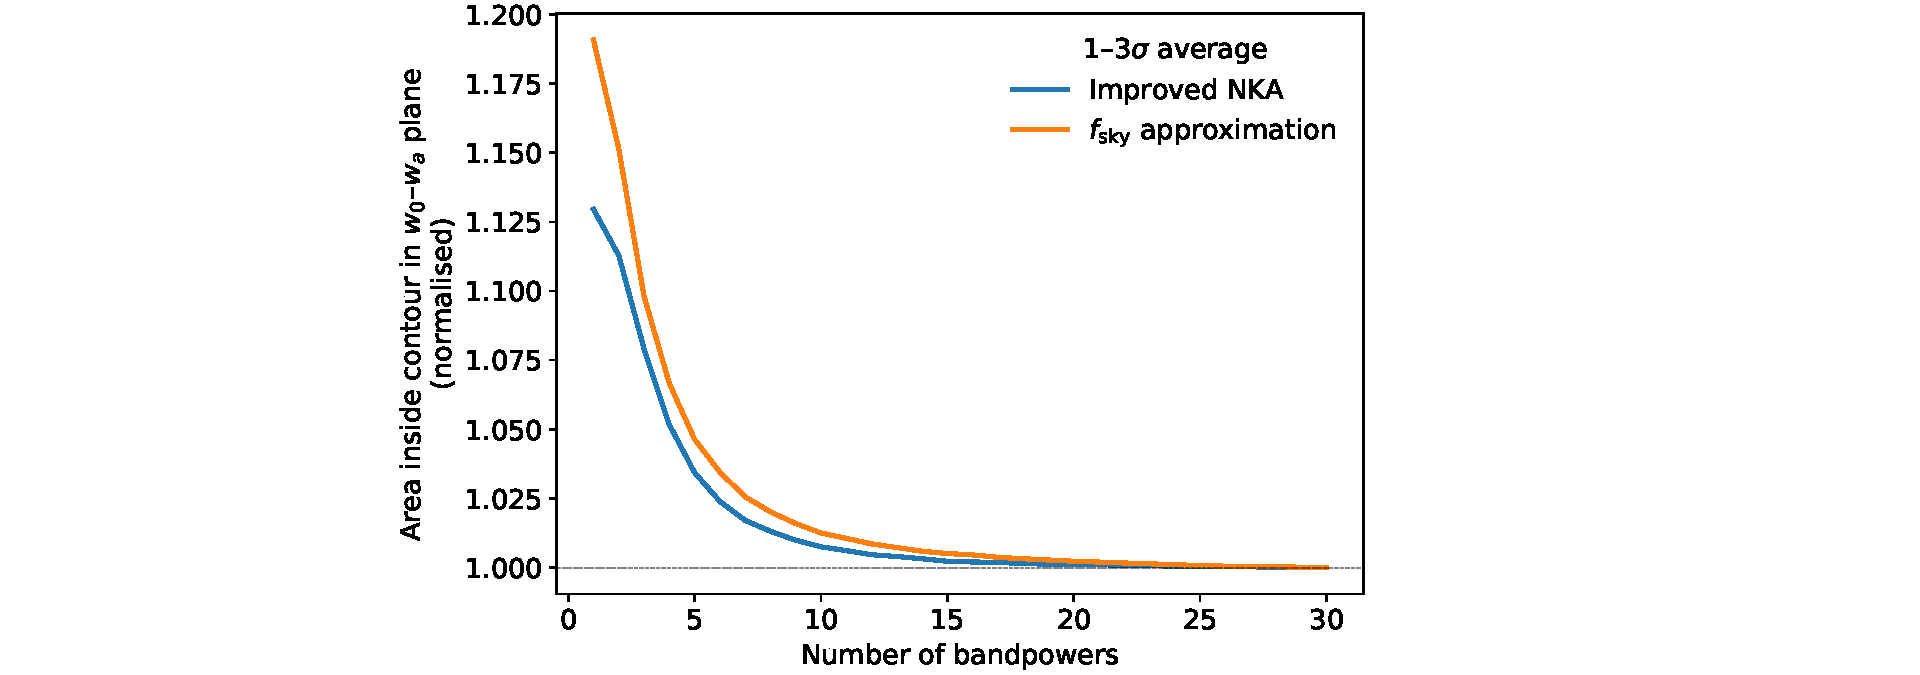
\includegraphics[width=\textwidth]{inka_vs_fsky}
\caption{Dependence of posterior uncertainties in a joint cut-sky analysis of $\wo$ and $\wa$ on the number of power spectrum bandpowers, when the covariance is calculated using the $\fsky$ approximation (\autoref{bin_eq:fsky_approx}) compared to the Improved NKA method. Each line is averaged over 100 contours linearly spaced from $1\sigma$ to $3\sigma$ and normalised to be equal to 1 at its minimum, as described in the first paragraph of \autoref{bin_sec:results}.}
\label{bin_Fig:inka_vs_fsky}
\end{figure}

In \autoref{bin_sec:main_analysis}, the cut-sky power spectrum covariance was calculated using the Improved NKA method. A faster alternative is to use the `$\fsky$ approximation':
\begin{equation}
\text{Cov}_\text{cut-sky} \approx \frac{1}{\fsky}
\text{Cov}_\text{full-sky},
\label{bin_eq:fsky_approx}
\end{equation}
where $\fsky$ is the observed fraction of the sky. \autoref{bin_Fig:inka_vs_fsky} shows the dependence of posterior uncertainties in a joint cut-sky analysis of $\wo$ and $\wa$ on the number of bandpowers when using the $\fsky$ approximation compared to the more accurate Improved NKA method.
% While not identical, the results are similar, except with only 1--2 angular bins.
While the curves produced by the two methods are not identical, the results are similar other than for a very coarse binning (1--2 angular bins).
The good performance of the $\fsky$ approximation for the power spectrum supports its use for the correlation function in \autoref{bin_sec:main_analysis}, especially when combined with the results of \citet{Cabre2007}, which show through a comparison with simulations that this approximation is much more accurate for the correlation function than it is for the power spectrum.

\subsection{Contrast between power spectrum and correlation function behaviour for small numbers of bins}
\label{bin_sec:low_nbin}

A peculiar result that occurs throughout \autoref{bin_sec:main_analysis} is that posterior uncertainties obtained through a power spectrum analysis tend to degrade much less for small numbers of angular bins than those obtained through a correlation function analysis. For example, in \autoref{bin_Fig:area_vs_nbin_fs}, even a single bandpower only returns a joint $\wo$--$\wa$ uncertainty around 20 per cent larger than with 30 bandpowers, whereas for the correlation function there is a sharp divergence by at least 500 per cent at around 5 angular bins. The explanation for this behaviour is the differing ways in which scales are weighted within each angular bin for the two methods, which will now be demonstrated.

\begin{figure}[t]
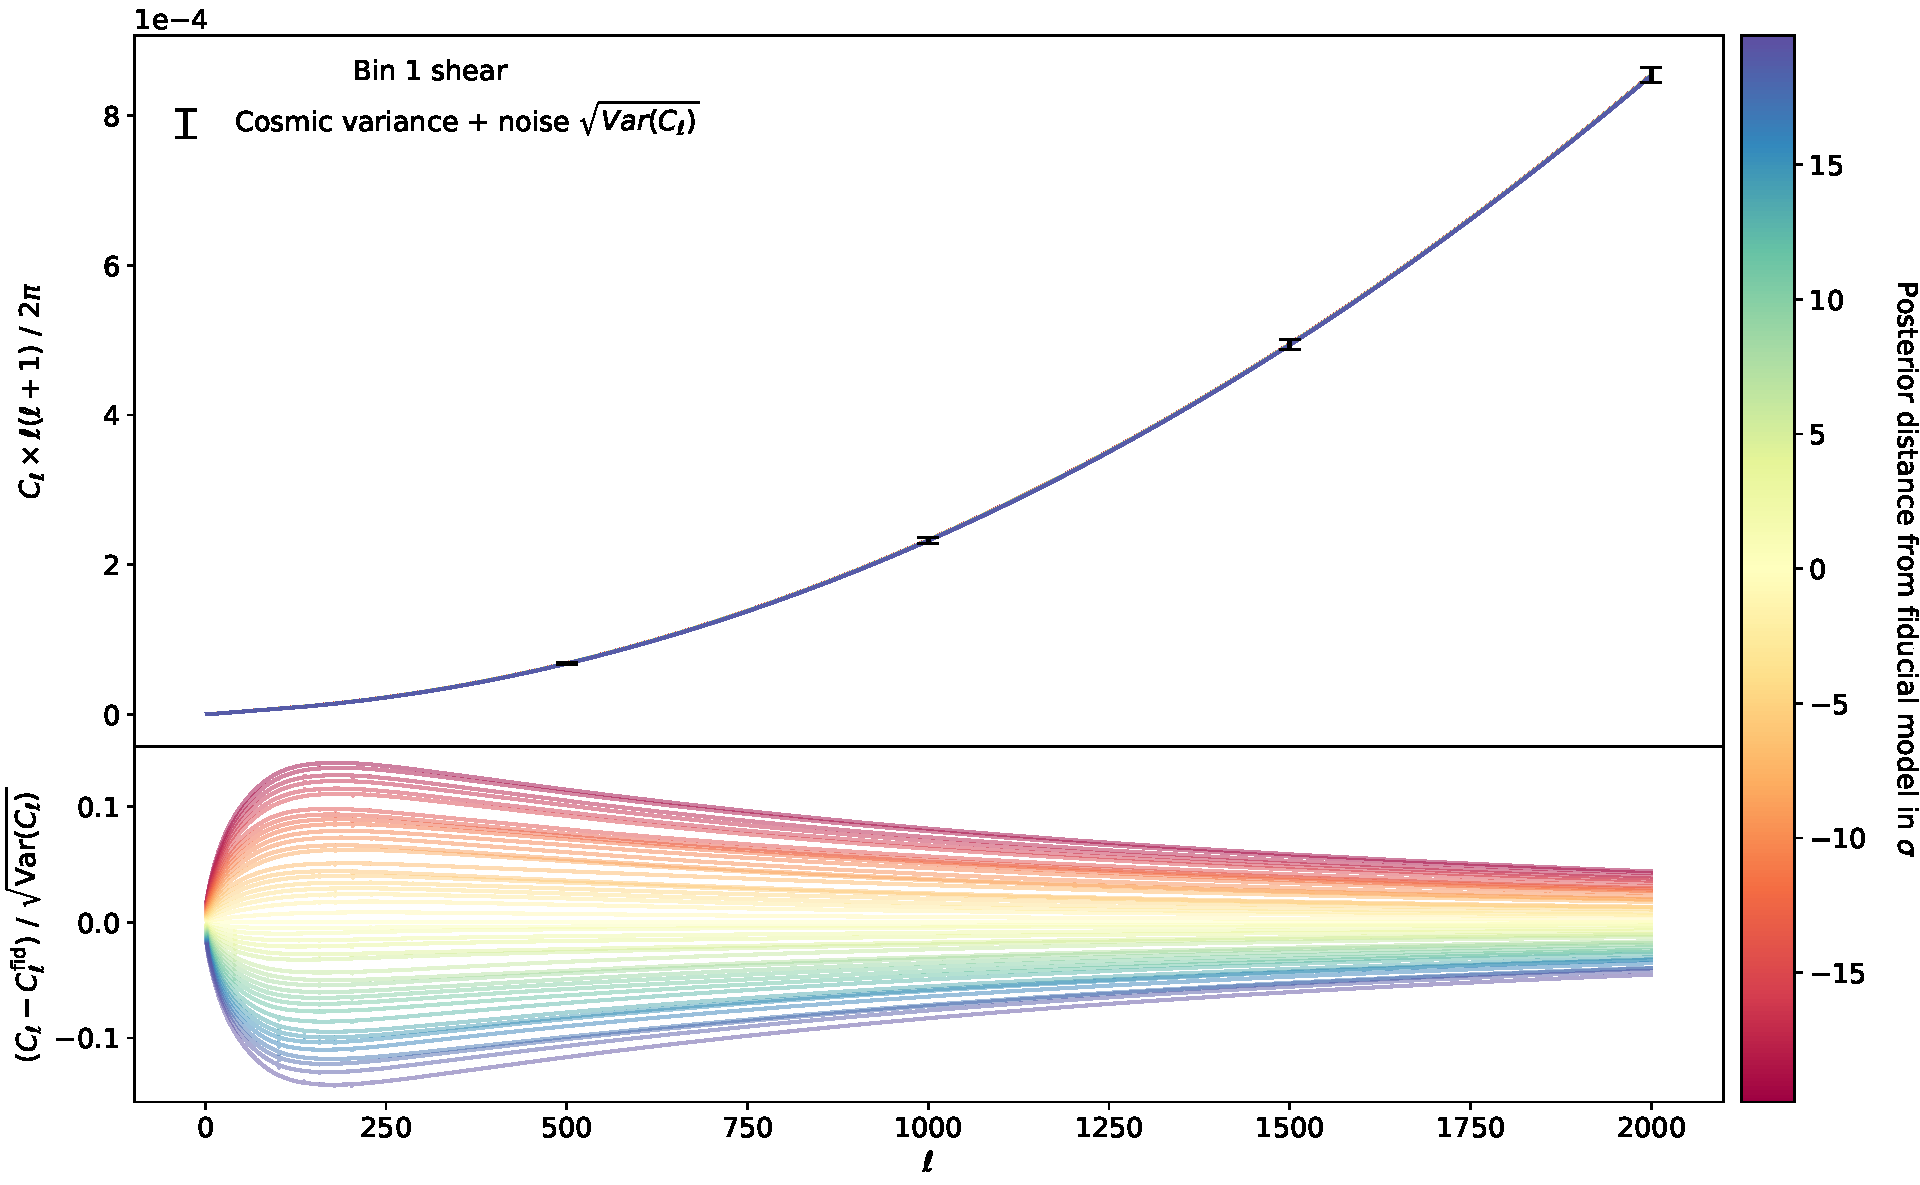
\includegraphics[width=\textwidth]{cl_perl}
\caption{Top: 45 theoretical power spectra, corresponding to the shear auto-power in the lowest redshift bin for different points in the $\wo$--$\wa$ plane. The points are chosen from a diagonal line running perpendicular to the $\wo$--$\wa$ degeneracy direction. Each model is coloured by its distance in $\sigma$ from the fiducial model, determined from a full-sky unbinned power spectrum likelihood analysis. In practice, the 45 power spectra all appear on top of one another. Error bars are shown at a selection of multipoles, and include a shape noise contribution. Bottom: The difference between each model and the fiducial model, scaled by the error bar for each $\ell$.}
\label{bin_Fig:cl_perl}
\end{figure}

The top panel of \autoref{bin_Fig:cl_perl} shows 45 theoretical power spectra, corresponding to the shear auto-power in the lowest redshift bin for different points in the $\wo$--$\wa$ plane. The points are chosen from a diagonal line running perpendicular to the $\wo$--$\wa$ degeneracy direction; that is, from the lower left to upper right of a given panel of \autoref{bin_Fig:posts_w0wa_cl}. Each model is coloured by its distance in $\sigma$ from the fiducial model, determined from a full-sky unbinned power spectrum likelihood analysis. The fiducial model is ($\wo$, $\wa$) = ($-1$, $0$). In practice, the 45 power spectra all appear on top of one another. Error bars are shown at a selection of multipoles, and include a shape noise contribution. In the lower panel, the difference between each model and the fiducial model is shown, scaled by the error bar for each $\ell$. This is effectively equivalent to the per-$\ell$ signal-to-noise as a function of scale. There is a region of very low signal-to-noise at low $\ell$, $\ell \lesssim 50$, which rapidly increases to a peak at around $\ell \sim 200$, followed by a gentle decrease towards higher $\ell$ as shape noise begins to dominate.

\begin{figure}[t]
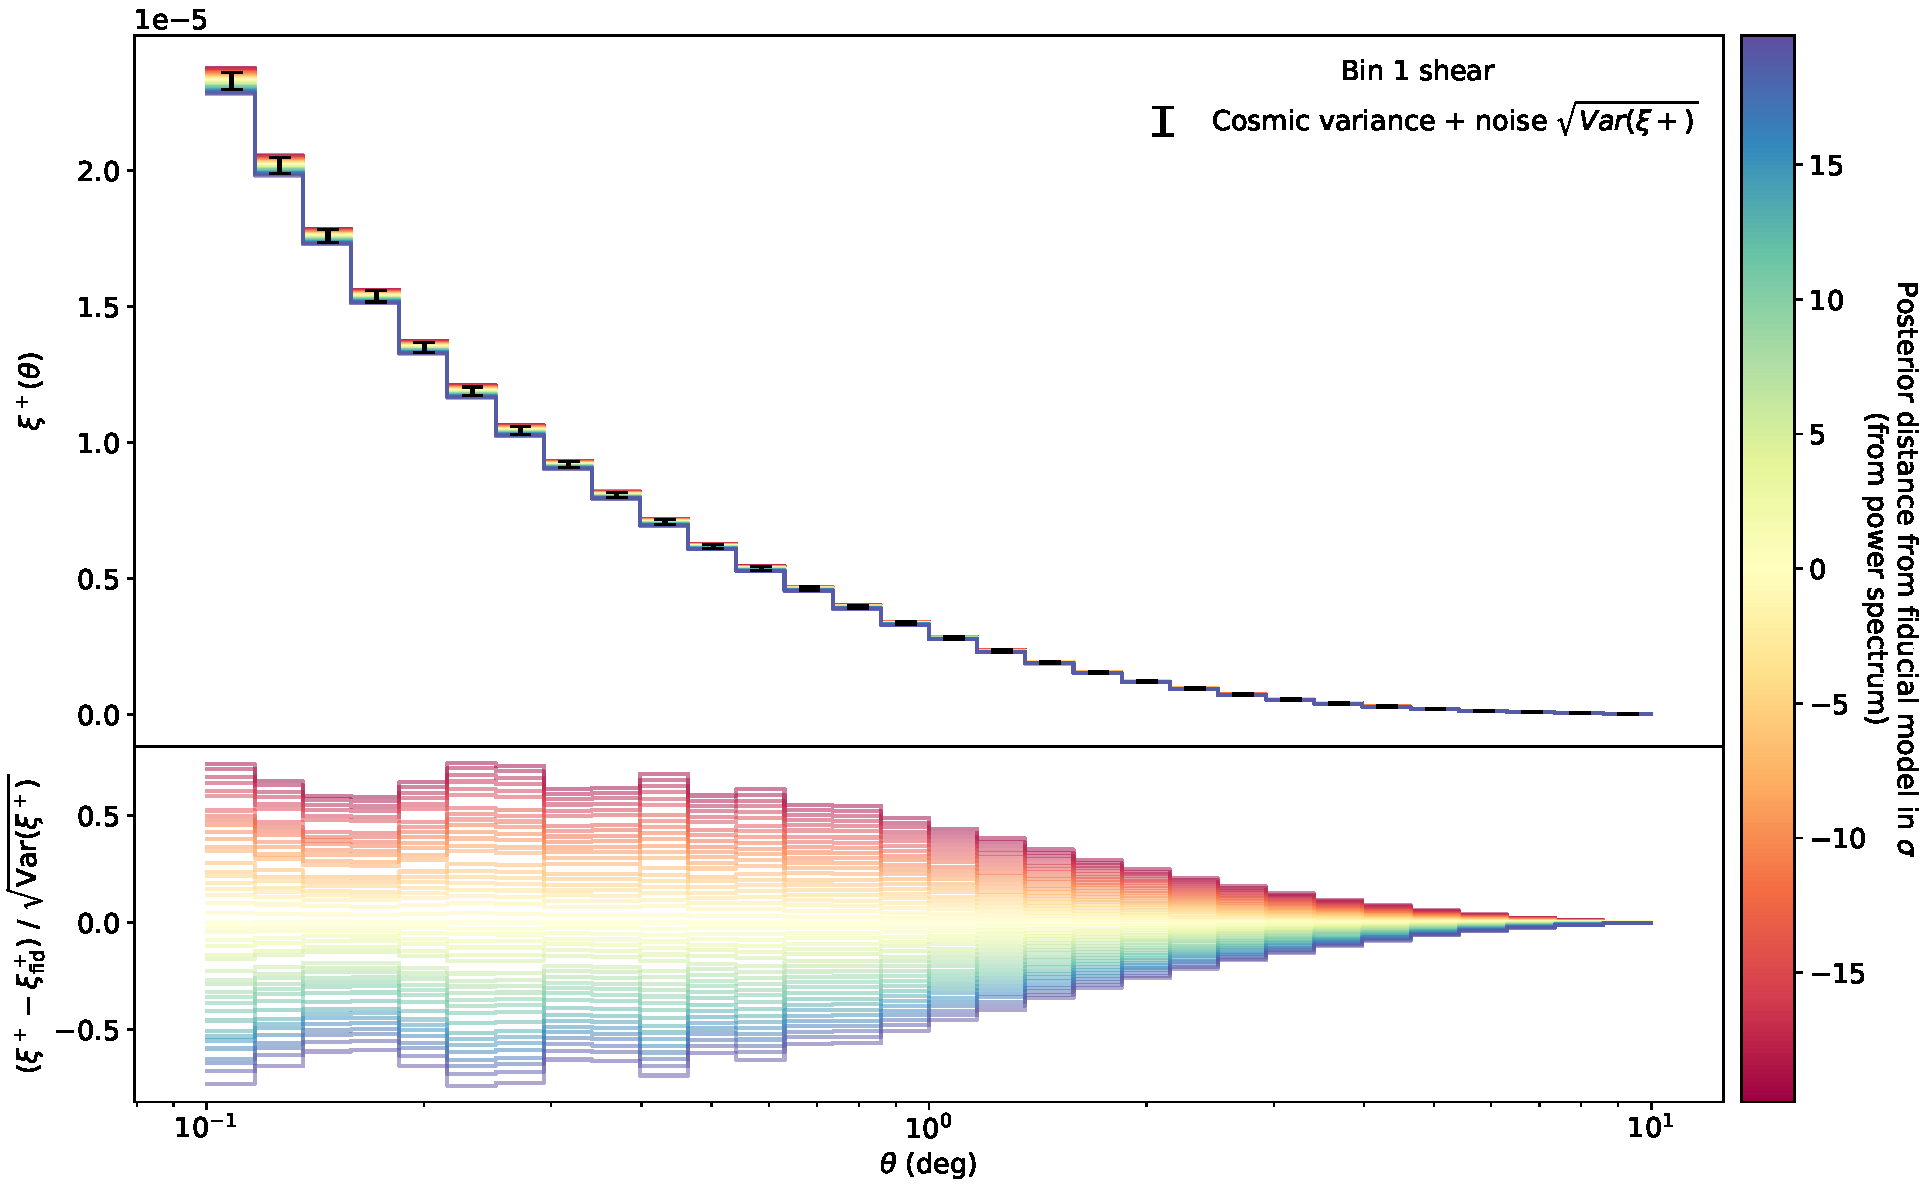
\includegraphics[width=\textwidth]{cf_perbin}
\caption{As \autoref{bin_Fig:cl_perl} but for the correlation function. Top: 45 theoretical correlation functions, corresponding to $\xi^+$ in the lowest redshift bin for different points in the $\wo$--$\wa$ plane. The points are chosen from a diagonal line running perpendicular to the $\wo$--$\wa$ degeneracy direction. Each model is coloured by its distance in $\sigma$ from the fiducial model, determined from a full-sky unbinned power spectrum likelihood analysis. Error bars are shown for each angular bin, and include a shape noise contribution. Bottom: The difference between each model and the fiducial model, scaled by the error bar for each angular bin.}
\label{bin_Fig:cf_perbin}
\end{figure}

The equivalent for the correlation function, for $\xi^+$ in the lowest redshift bin, is shown in \autoref{bin_Fig:cf_perbin}. 30 angular bins are used. The colour for each model is the same as in \autoref{bin_Fig:cl_perl}. The signal-to-noise is roughly constant between 0.1 and 1 deg, before steadily decreasing to reach a very low level at 10 deg.

As seen in Figures \ref{bin_Fig:cl_perl} and \ref{bin_Fig:cf_perbin}, both the power spectrum and correlation function have poor signal-to-noise on large angular scales. This fact alone cannot explain the difference between them when small numbers of angular bins are used. The difference arises because of how scales are weighted within each bin. For the power spectrum, different $\ell$ within each bandpower are weighted as $\ell \left( \ell + 1 \right)$ following Equation \eqref{cov_eqn:pbl}, which quadratically downweights the largest scales, which are the lowest signal-to-noise part of the data vector. For the correlation function, however, different $\theta$ within each bin are weighted as $\sin{\theta}$, corresponding to a uniform distribution of galaxies \citep{Friedrich2021}. This weighting upweights the largest scales, which can dramatically decrease the signal-to-noise when combining scales into few bins.

\begin{figure}[tp]
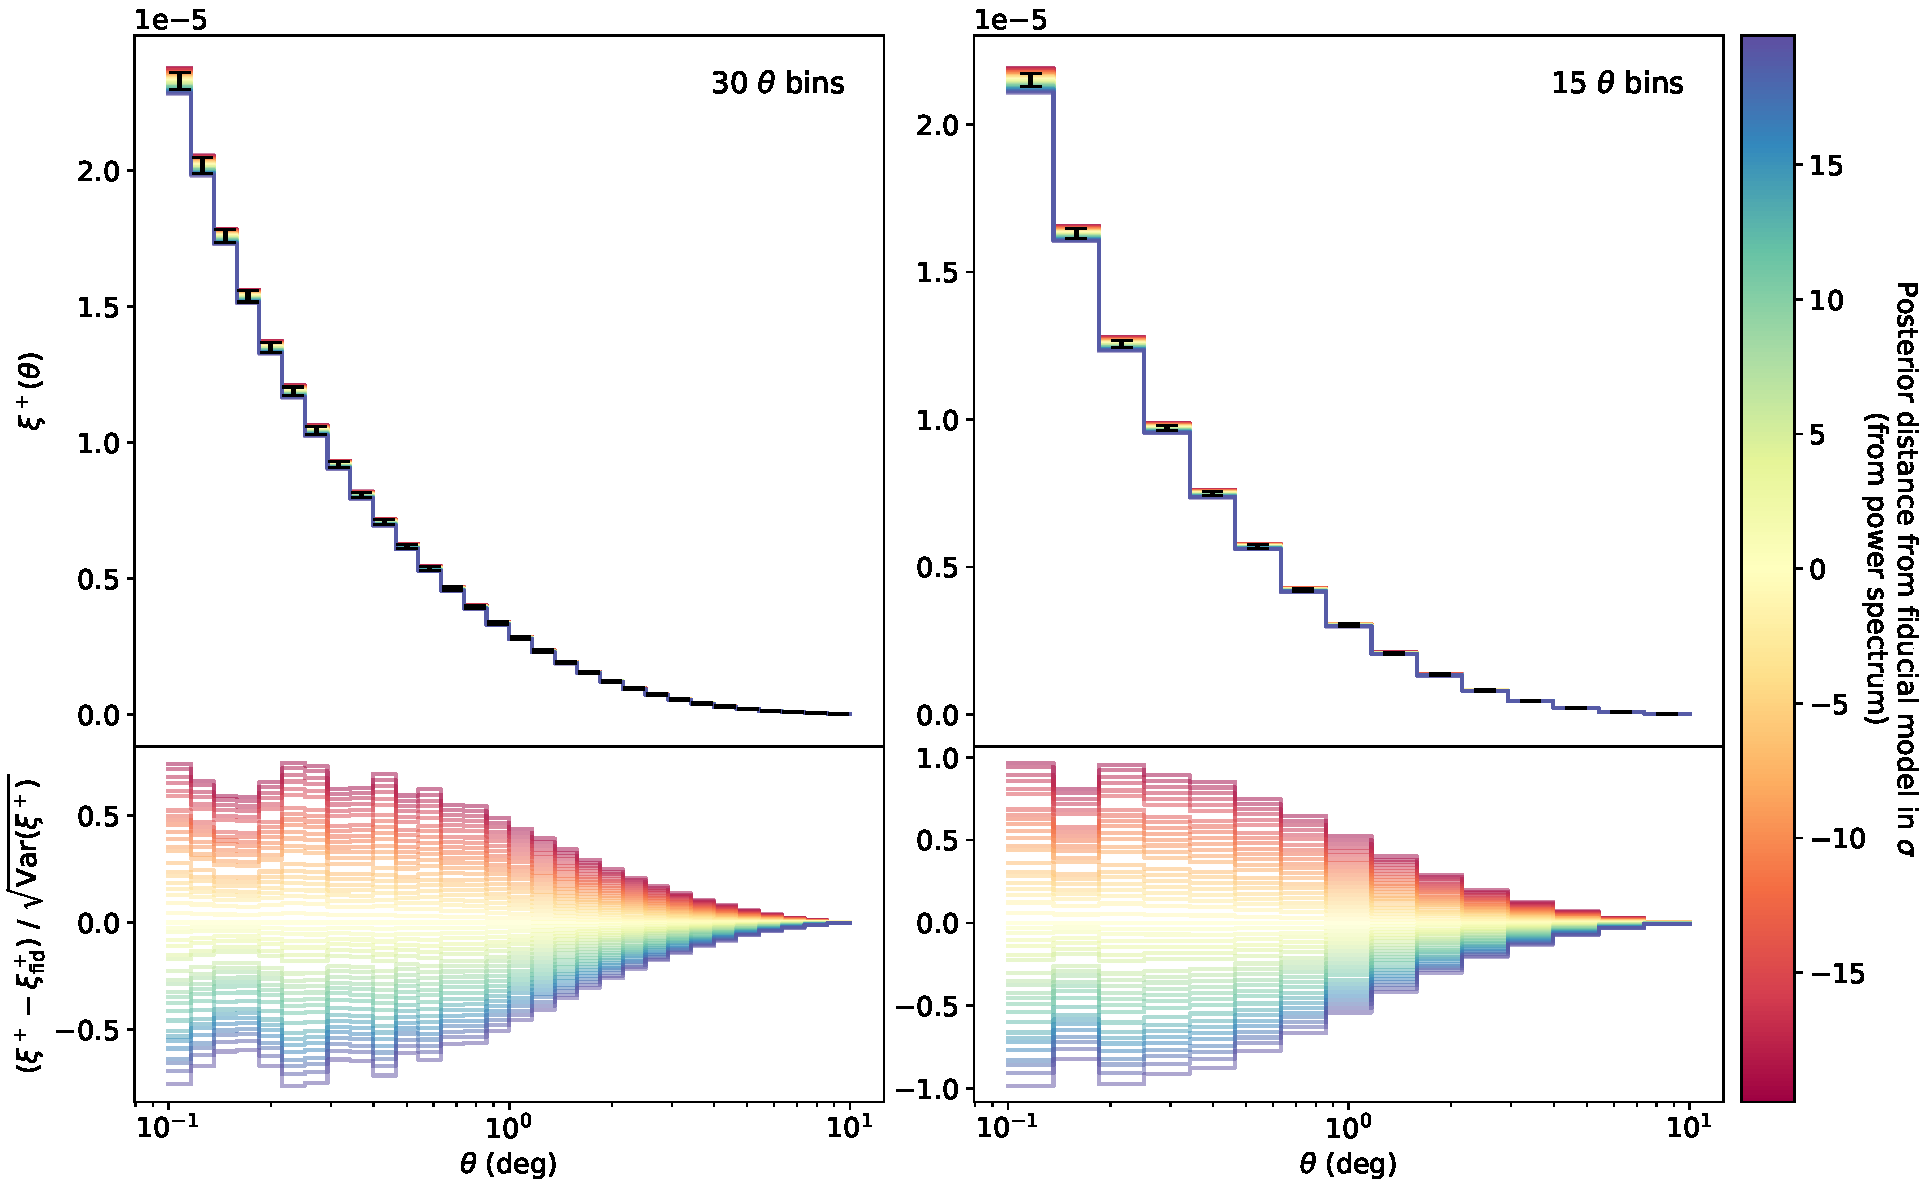
\includegraphics[width=\textwidth]{cf_perbin_30vs15}
\caption{As \autoref{bin_Fig:cf_perbin}, but for 30 angular bins (left panel) compared to 15 (right panel).}
\label{bin_Fig:cf_perbin_30vs15}
\end{figure}

\begin{figure}[tp]
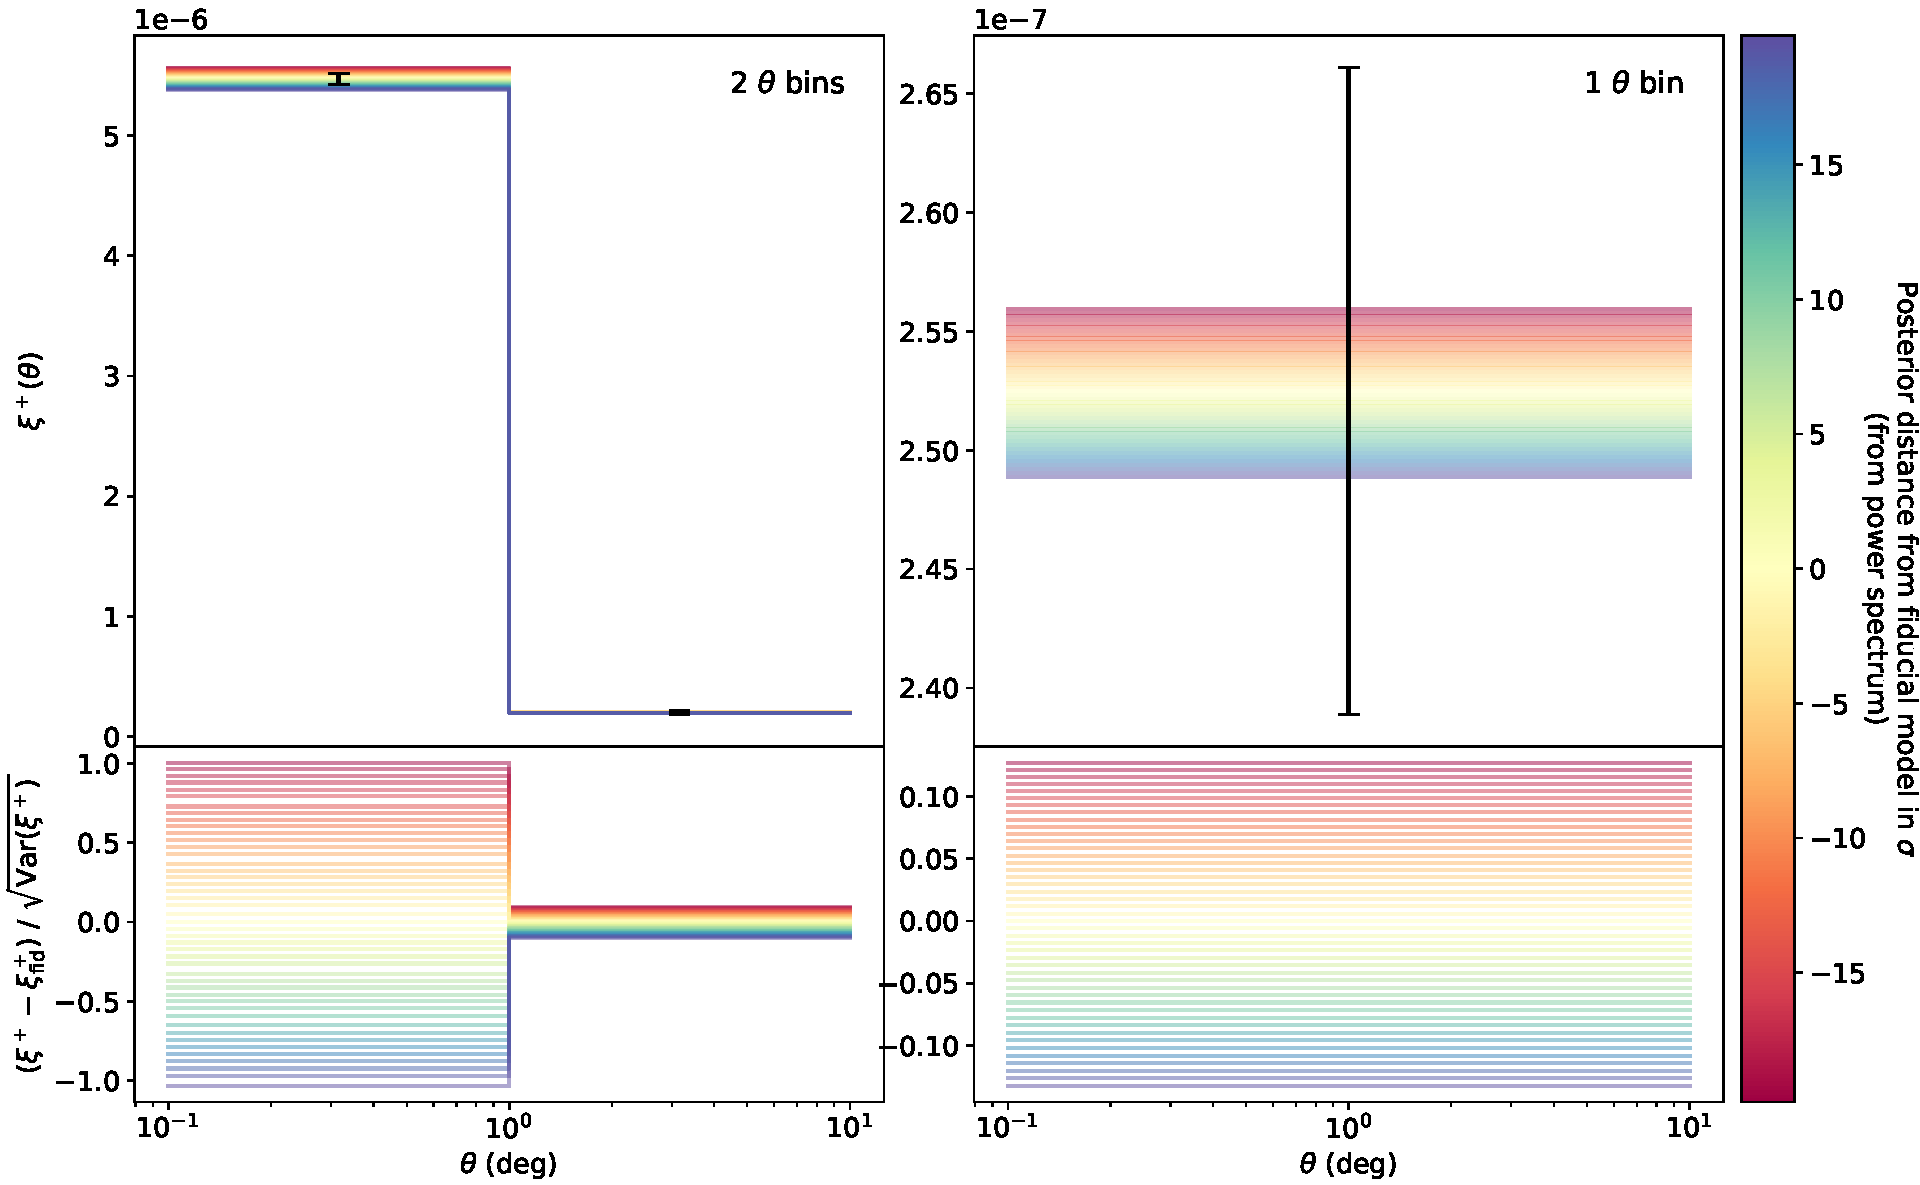
\includegraphics[width=\textwidth]{cf_perbin_2vs1}
\caption{As \autoref{bin_Fig:cf_perbin}, but for 2 angular bins (left panel) compared to 1 (right panel).}
\label{bin_Fig:cf_perbin_2vs1}
\end{figure}

The effect of the $\sin{\theta}$ weighting is small when relatively large numbers of angular bins are used. The left panel of \autoref{bin_Fig:cf_perbin_30vs15} shows the same selection of correlation functions and per-bin signal-to-noise for 30 angular bins, while the right panel uses 15 bins. Each angular bin on the right panel corresponds to exactly two bins on the left panel. It can be seen that the $\sin{\theta}$ weighting has little effect, because for instance the value of $\xi^+$ in the first bin in the right panel is approximately equal to the mean of the values of $\xi^+$ in the first two bins in the left panel. This is because with a fine binning such as that used here, the difference in $\sin{\theta}$ between adjacent bins is not significant.

However, with a very low number of bins the effect of the $\sin{\theta}$ weighting is large. \autoref{bin_Fig:cf_perbin_2vs1} shows the difference between using two angular bins in the left panel and just a single bin in the right panel. When combining the two bins into one, the value of $\xi^+$ is heavily weighted towards the larger-scale bin. The result is that the signal-to-noise drops by an order of magnitude, as is evident in the lower panels.

It is possible to demonstrate that the power spectrum would experience the same problem if large scales were not strongly downweighted. To do so, it is necessary to introduce a new technique, in order to combine the signal-to-noise across all angular bins while taking correlations between bins into account. This involves defining the covariance-weighted distance $d$,\footnote{This distance $d$ is equivalent to the Mahalanobis distance
\citep{Mahalanobis1936}.} as
\begin{equation}
d^2 = \left( \mathbf{x} - \mathbf{x}^\text{fid} \right)^\intercal
\mathbfss{\Sigma}^{-1}
\left( \mathbf{x} - \mathbf{x}^\text{fid} \right),
\label{bin_eq:cov_dist}
\end{equation}
where $\mathbf{x}$ is the theoretical data vector for a particular model (a set of $\Cl$ or $\xi \left( \theta \right)$ values), $\mathbf{x}^\text{fid}$ is the data vector predicted by the fiducial model, and $\mathbfss{\Sigma}$ is the covariance matrix.

\begin{figure}[tp]
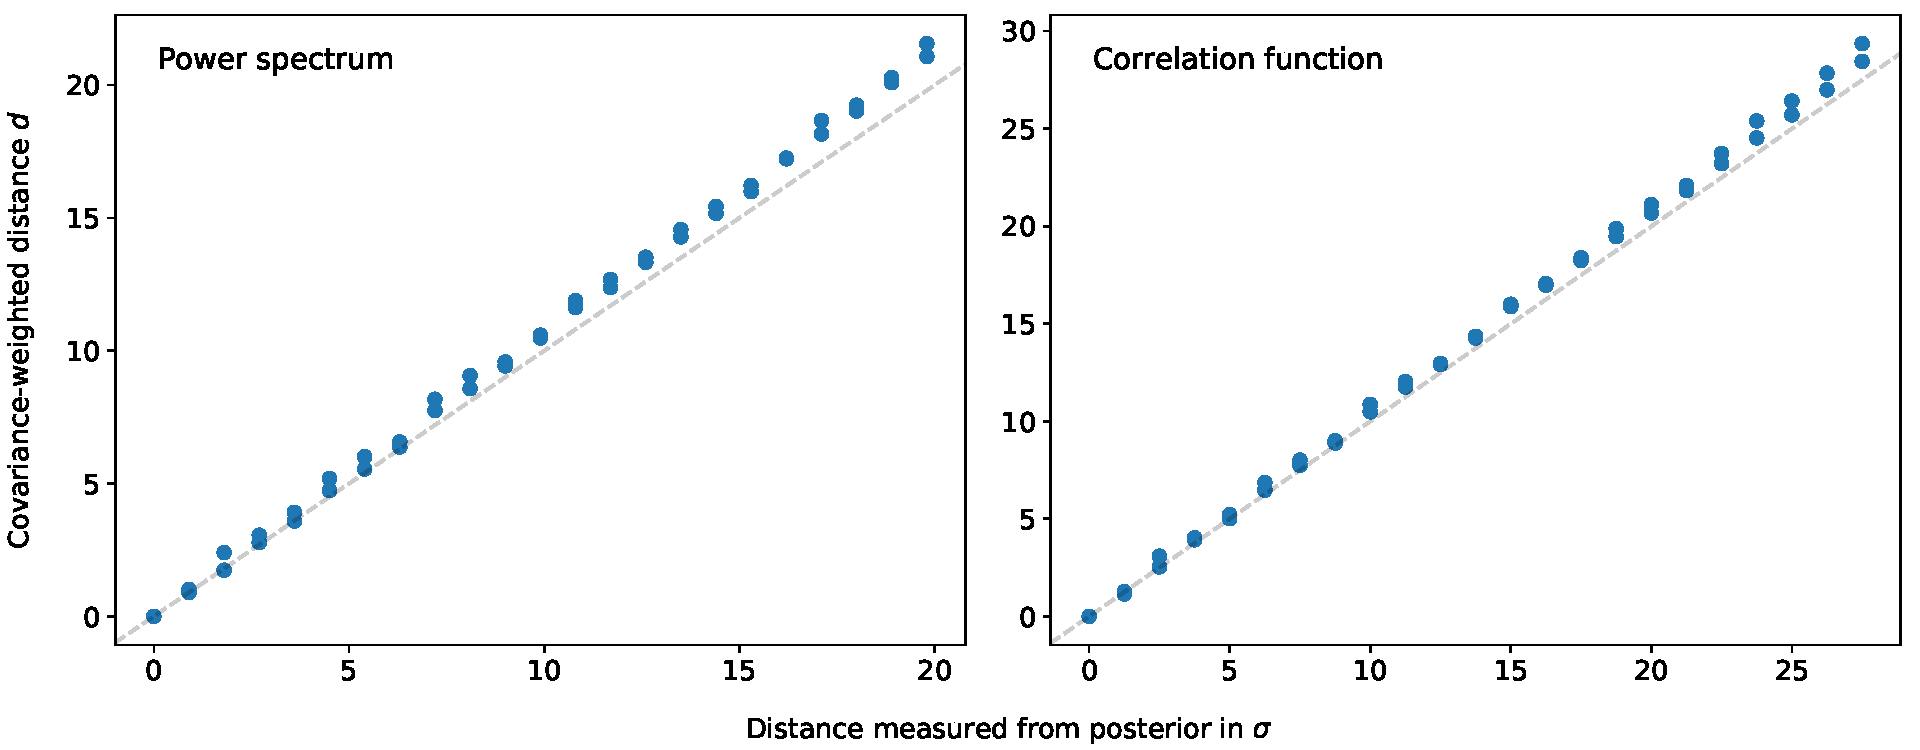
\includegraphics[width=\textwidth]{dist_validation}
\caption{Comparison of the covariance-weighted distance $d$ defined in \eqref{bin_eq:cov_dist} to the distance from the fiducial model measured from the posterior distribution resulting from a full likelihood analysis, for each of 45 different models. Each model corresponds to a different point in the $\wo$-$\wa$ plane, selected from a diagonal line running perpendicular to the $\wo$--$\wa$ degeneracy direction. The dashed line represents equality.}
\label{bin_Fig:dist_validation}
\end{figure}

\autoref{bin_Fig:dist_validation} shows that Equation \eqref{bin_eq:cov_dist} correctly predicts the distance from the fiducial model measured from the posterior distribution resulting from a full likelihood analysis. The left panel shows the value of the covariance-weighted distance $d$ against the distance from the fiducial model in $\sigma$ measured from the posterior for the power spectrum, while the right panel shows it for the correlation function, for the selection of 45 models used throughout this section. The agreement is worse farther from the fiducial model, which may be a result of being close to the boundary of the prior region used in the likelihood analysis.

\begin{figure}[tp]
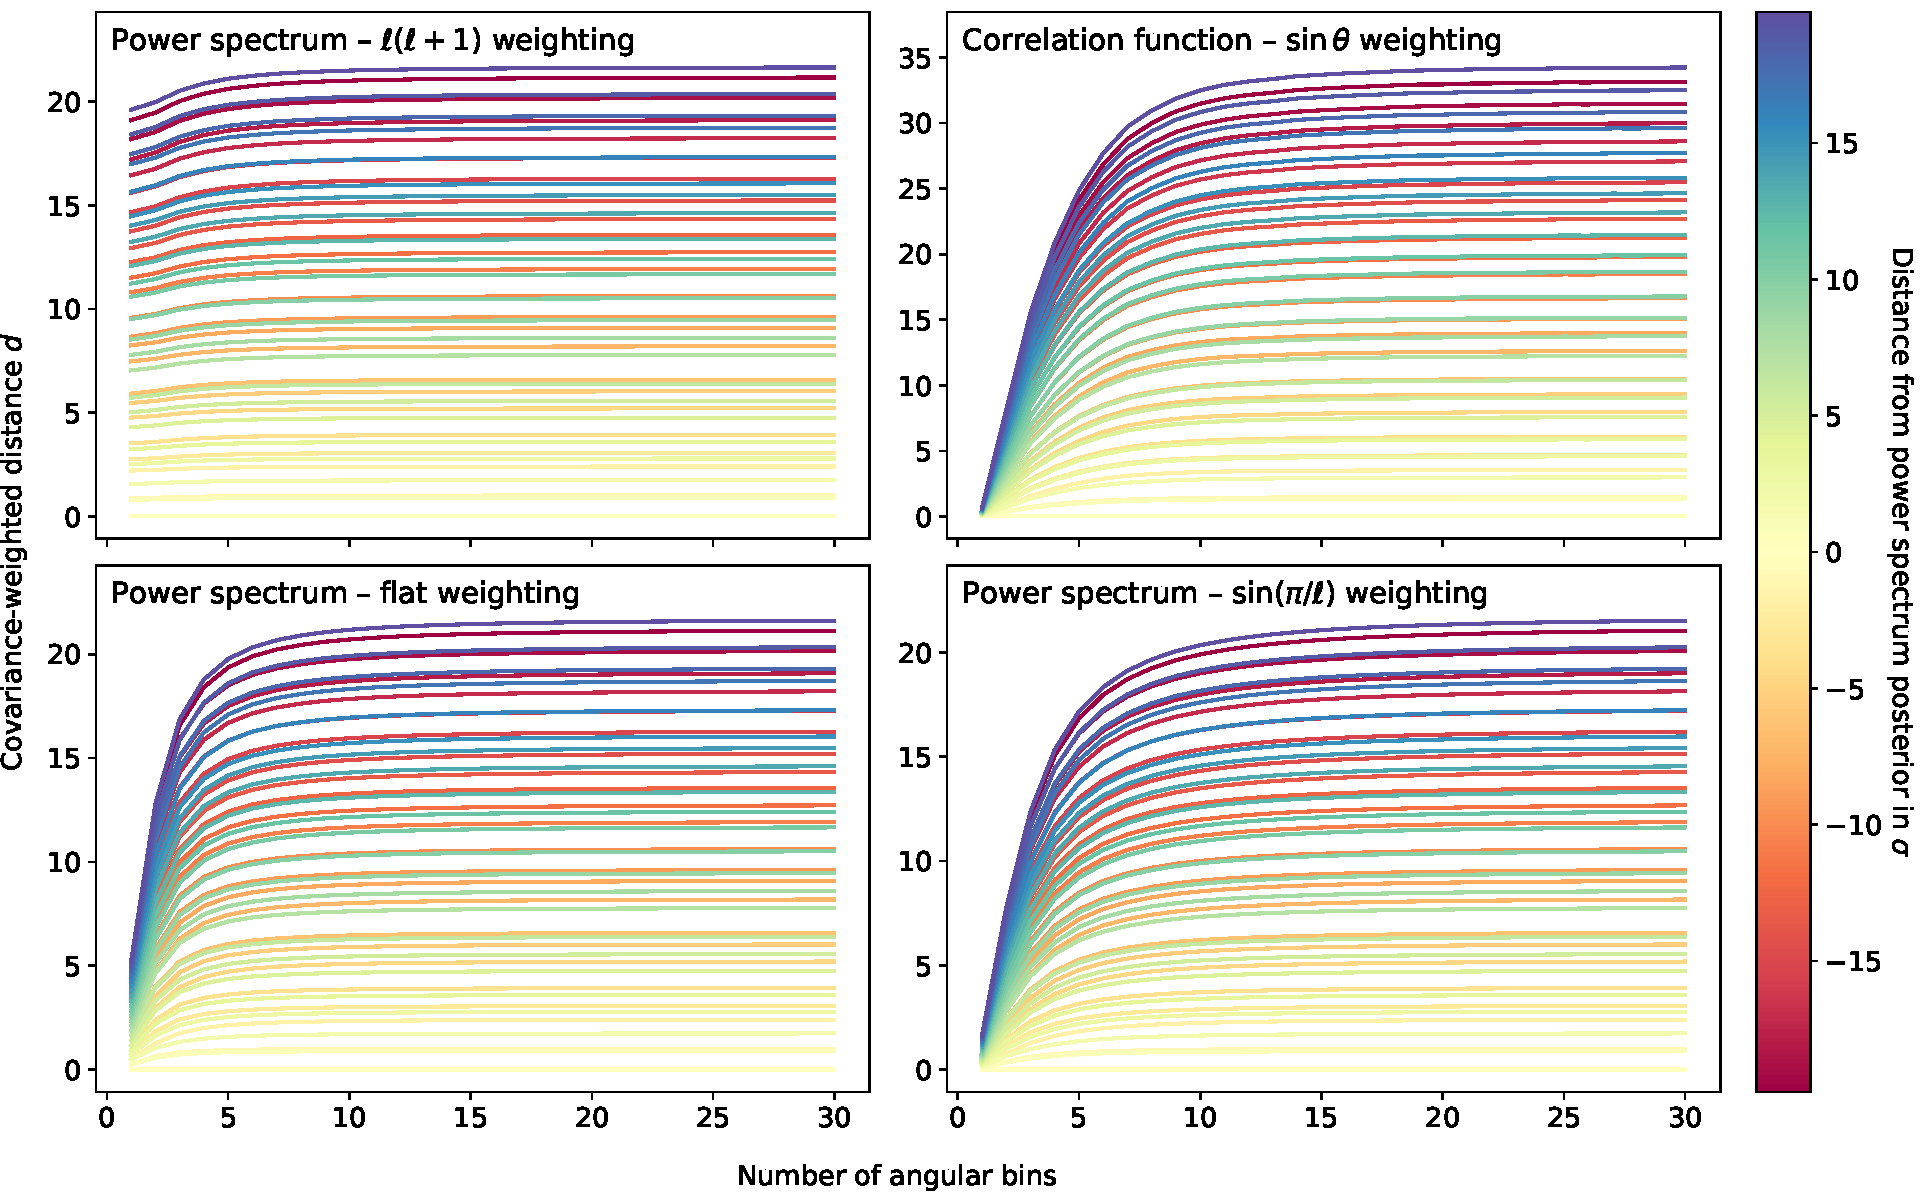
\includegraphics[width=\textwidth]{dist_weight}
\caption{Covariance-weighted distance $d$ from the fiducial model, as defined in Equation \eqref{bin_eq:cov_dist}, as a function of the number of angular bins, for a selection of 45 different models. Each model corresponds to a different point in the $\wo$-$\wa$ plane, selected from a diagonal line running perpendicular to the $\wo$--$\wa$ degeneracy direction. Each panel explores a different weighting of scales within each angular bin. Top left: power spectrum with the usual $\ell \left( \ell + 1 \right)$ weighting. Top right: correlation function with the $\sin{\theta}$ weighting corresponding to a uniform distribution of galaxies. Bottom left: power spectrum with a flat weighting, where each $\ell$ is weighted equally within each bandpower. Bottom right: power spectrum with a correlation-function-like $\sin{\left( \pi / \ell \right)}$ weighting.}
\label{bin_Fig:dist_weight}
\end{figure}

The upper left panel of \autoref{bin_Fig:dist_weight} shows the covariance-weighted distance from the fiducial model as a function of the number of angular bins for the power spectrum with the usual $\ell \left( \ell + 1 \right)$ weighting, for each of the 45 models. The results are consistent with those found from a full likelihood analysis in \autoref{bin_Fig:area_vs_nbin_fs}: the distance at which each model is excluded only decreases slightly when reducing the number of bandpowers, even to a single bandpower. The upper right panel shows the equivalent for the correlation function, which is weighted within each bin as $\sin{\theta}$. As seen previously in \autoref{bin_Fig:area_vs_nbin_fs}, there is a much more severe degradation in performance for small numbers of bins, with the distance from the fiducial model shrinking to approximately zero for a model excluded at more than 30$\sigma$ with 20--30 angular bins.

The lower left panel of \autoref{bin_Fig:dist_weight} shows the effect of applying a flat weighting to the power spectrum; that is, weighting each $\ell$ equally within a given bandpower. The effect here is to reduce the amount by which large scales are downweighted, which leads to a degradation in the overall signal-to-noise for small numbers of bandpowers. Finally, in the lower right panel, a weighting is applied that is equivalent to the way in which the correlation function is weighted: each $\ell$ is weighted as $\sin{\left( \pi / \ell \right)}$. The resulting form of the distance from the fiducial model as a function of the number of bins is almost identical to that for the correlation function. This demonstrates that the weighting of scales within bins is responsible for the different behaviour of the power spectrum and the correlation function for low numbers of angular bins.

\subsection{Impact of noise}
\label{bin_Sec:noise}

It is possible that the results derived in the main analysis presented in \autoref{bin_sec:main_analysis} may vary if the level of noise present in the data changes. This is investigated in this section.

\begin{figure}[tp]
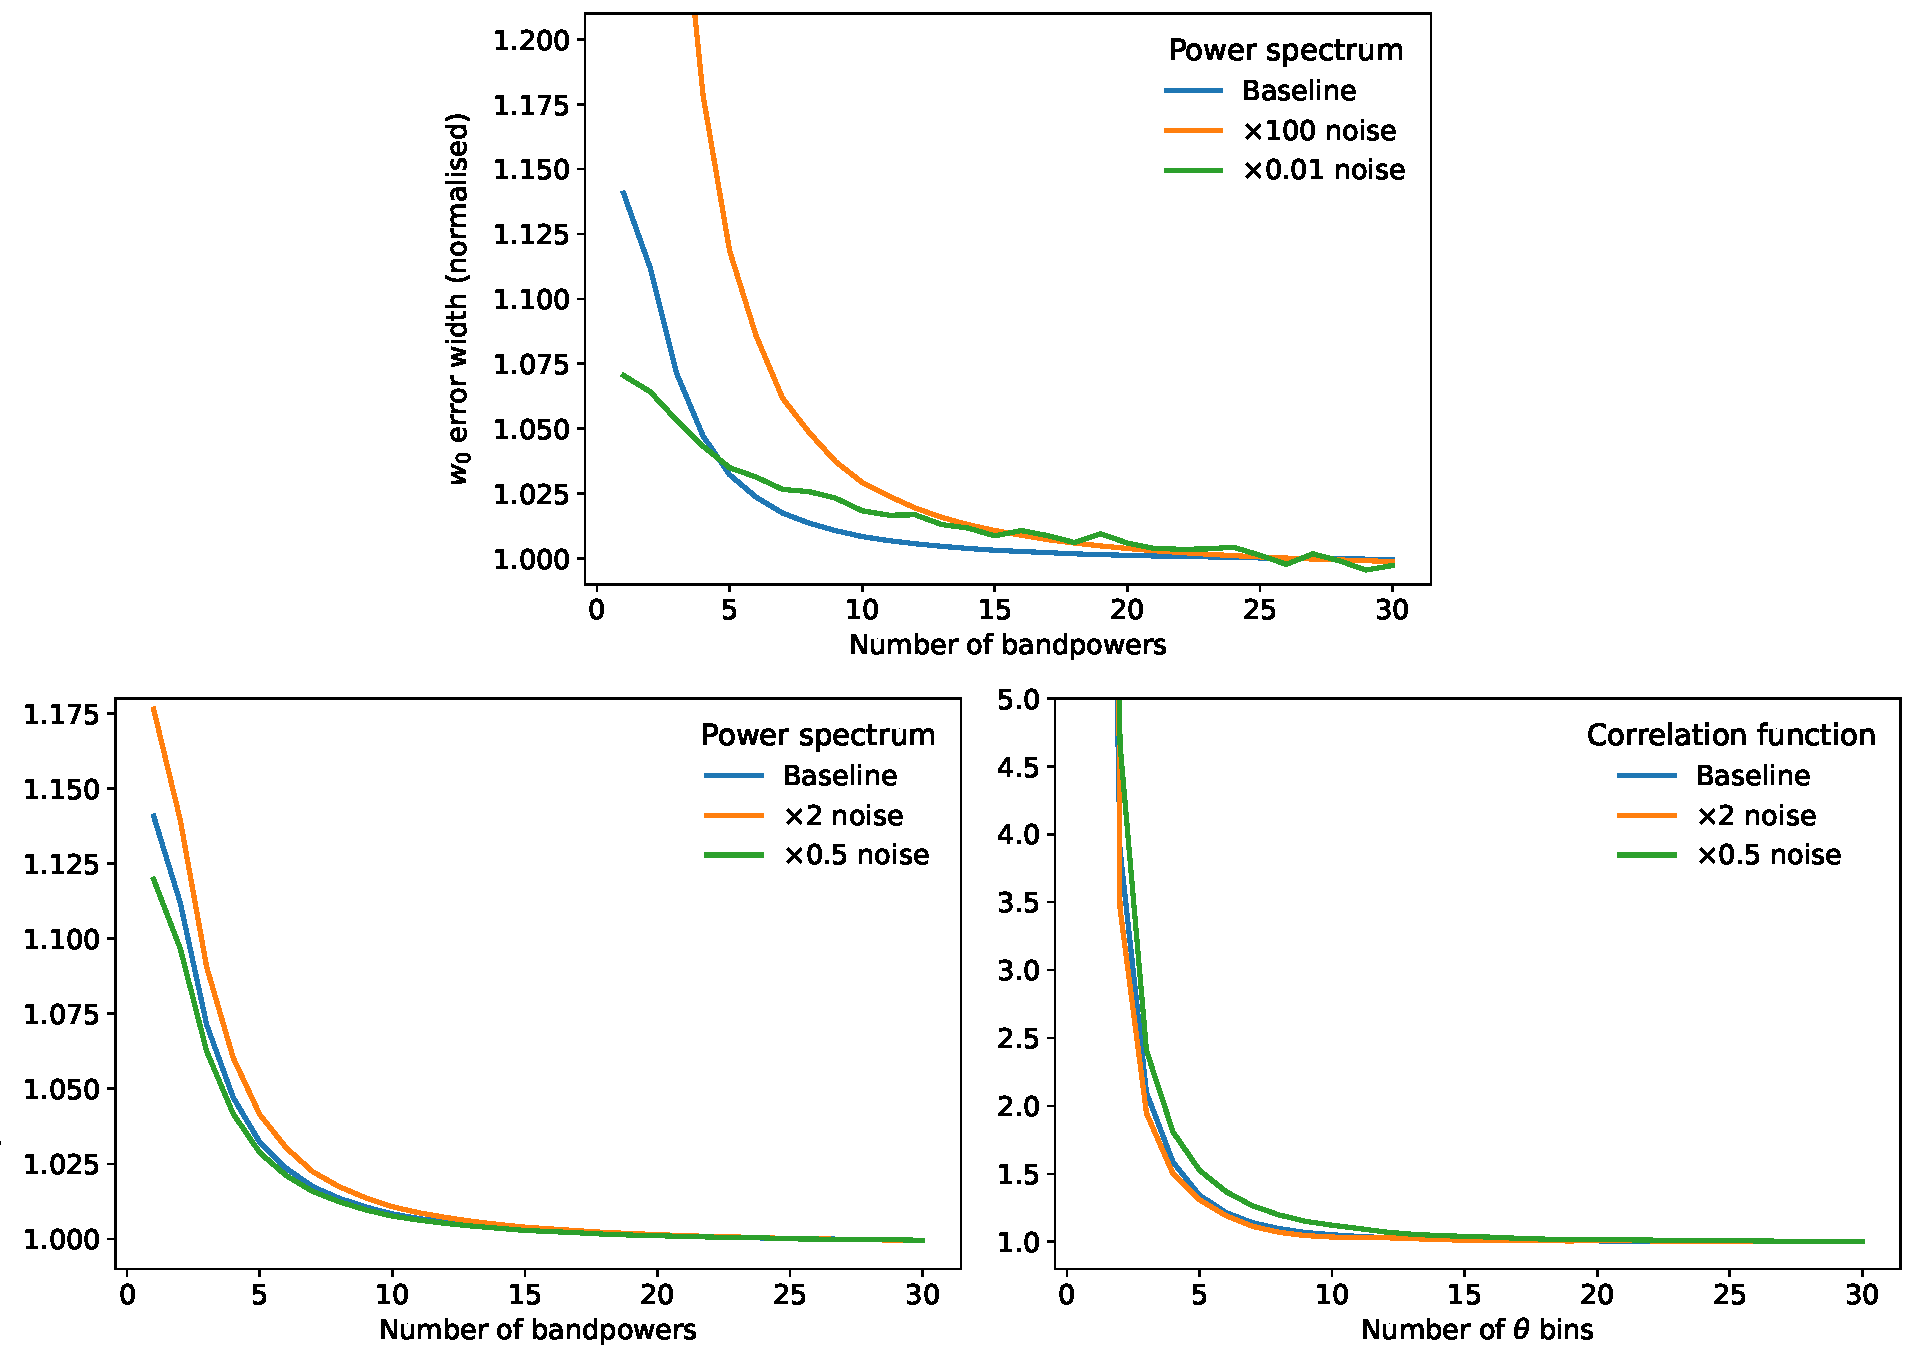
\includegraphics[width=\textwidth]{width_vs_noise}
\caption{Dependence of $\wo$ posterior uncertainty on the number of angular bins for the power spectrum and correlation function, for three different noise levels. Top: power spectrum, varying noise by a factor of 100. Lower left: power spectrum, varying noise by a factor of 2. Lower right: correlation function, varying noise by a factor of 2. Each line is averaged over 100 contours linearly spaced from $1\sigma$ to $3\sigma$ and normalised to be equal to 1 at its minimum, as described in the first paragraph of \autoref{bin_sec:results}. The baseline noise level corresponds to 30 galaxies\,/\,arcmin${}^2$ across all redshift bins.}
\label{bin_Fig:width_vs_noise}
\end{figure}

The top panel of \autoref{bin_Fig:width_vs_noise} shows the posterior uncertainty in $\wo$ from a full-sky power spectrum analysis, as a function of the number of bandpowers, for three noise levels. The baseline noise level corresponds to 30 galaxies\,/\,arcmin${}^2$ across all redshift bins, while the line labelled `$\times$100 noise' corresponds to 0.3\,/\,arcmin${}^2$ and the line labelled `$\times$0.01 noise' corresponds to 3000\,/\,arcmin${}^2$. Different behaviour is observed for the three different noise levels, which is discussed further below. Varying the noise by a factor 100 turned out to not be possible for the correlation function, due to problems with the conditioning of the covariance matrix for low noise levels. For a fair comparison with the correlation function, the lower left panel therefore shows the results for power spectrum with the noise varying by a factor of 2. `$\times$2 noise' corresponds to 15 galaxies\,/\,arcmin${}^2$, while `$\times$0.5 noise' corresponds to 60\,/\,arcmin${}^2$. While the spacing between the three lines is smaller than in the top panel, it is still clearly present in the same arrangement.

The right panel of \autoref{bin_Fig:width_vs_noise} shows the equivalent figure for the correlation function, with a factor of 2 between each noise level. In this case, little clear difference is observed between the different noise levels.

Insight into the different behaviour of the power spectrum and correlation function under varying noise levels seen in \autoref{bin_Fig:width_vs_noise} may be gained by studying the signal-to-noise as a function of scale for each method with an enhanced level of noise. This may be studied using some of the methods developed in \autoref{bin_sec:low_nbin} above. Since the methods used here do not require the use of a covariance matrix, a factor of 100$\times$ may be used without any problems, which allows a clearer illustration of the effect of noise.

The lower panel of \autoref{bin_Fig:cl_perl_x100noise} shows the per-$\ell$ signal-to-noise of the shear auto-power spectrum in the lowest redshift bin for the 100$\times$ baseline noise level. (See \autoref{bin_sec:low_nbin} for a more detailed explanation of this type of figure.) In contrast to the relatively small drop in signal-to-noise towards higher $\ell$ seen in \autoref{bin_Fig:cl_perl}, there is now a much larger decrease, in addition to a shift in the peak towards lower $\ell$ ($\ell \sim 50$). This is because the smaller scales are heavily suppressed by the increased noise level. If these low signal-to-noise small scales are combined in a single bin with the high signal-to-noise region, they will be strongly upweighted by the $\ell \left( \ell + 1 \right)$ weighting of $\ell$s within bandpowers, leading to a strong decrease in the overall signal-to-noise. This is what is observed in the `$\times$100 noise' line in the top panel of \autoref{bin_Fig:width_vs_noise}, and to a smaller extend in the `$\times$2 noise' line in the lower left panel of the same figure. The opposite effect can be expected to occur for low noise levels, which can explain the shallow slope of the `$\times$0.01 noise' and `$\times$0.5 noise' lines.

\begin{figure}[tp]
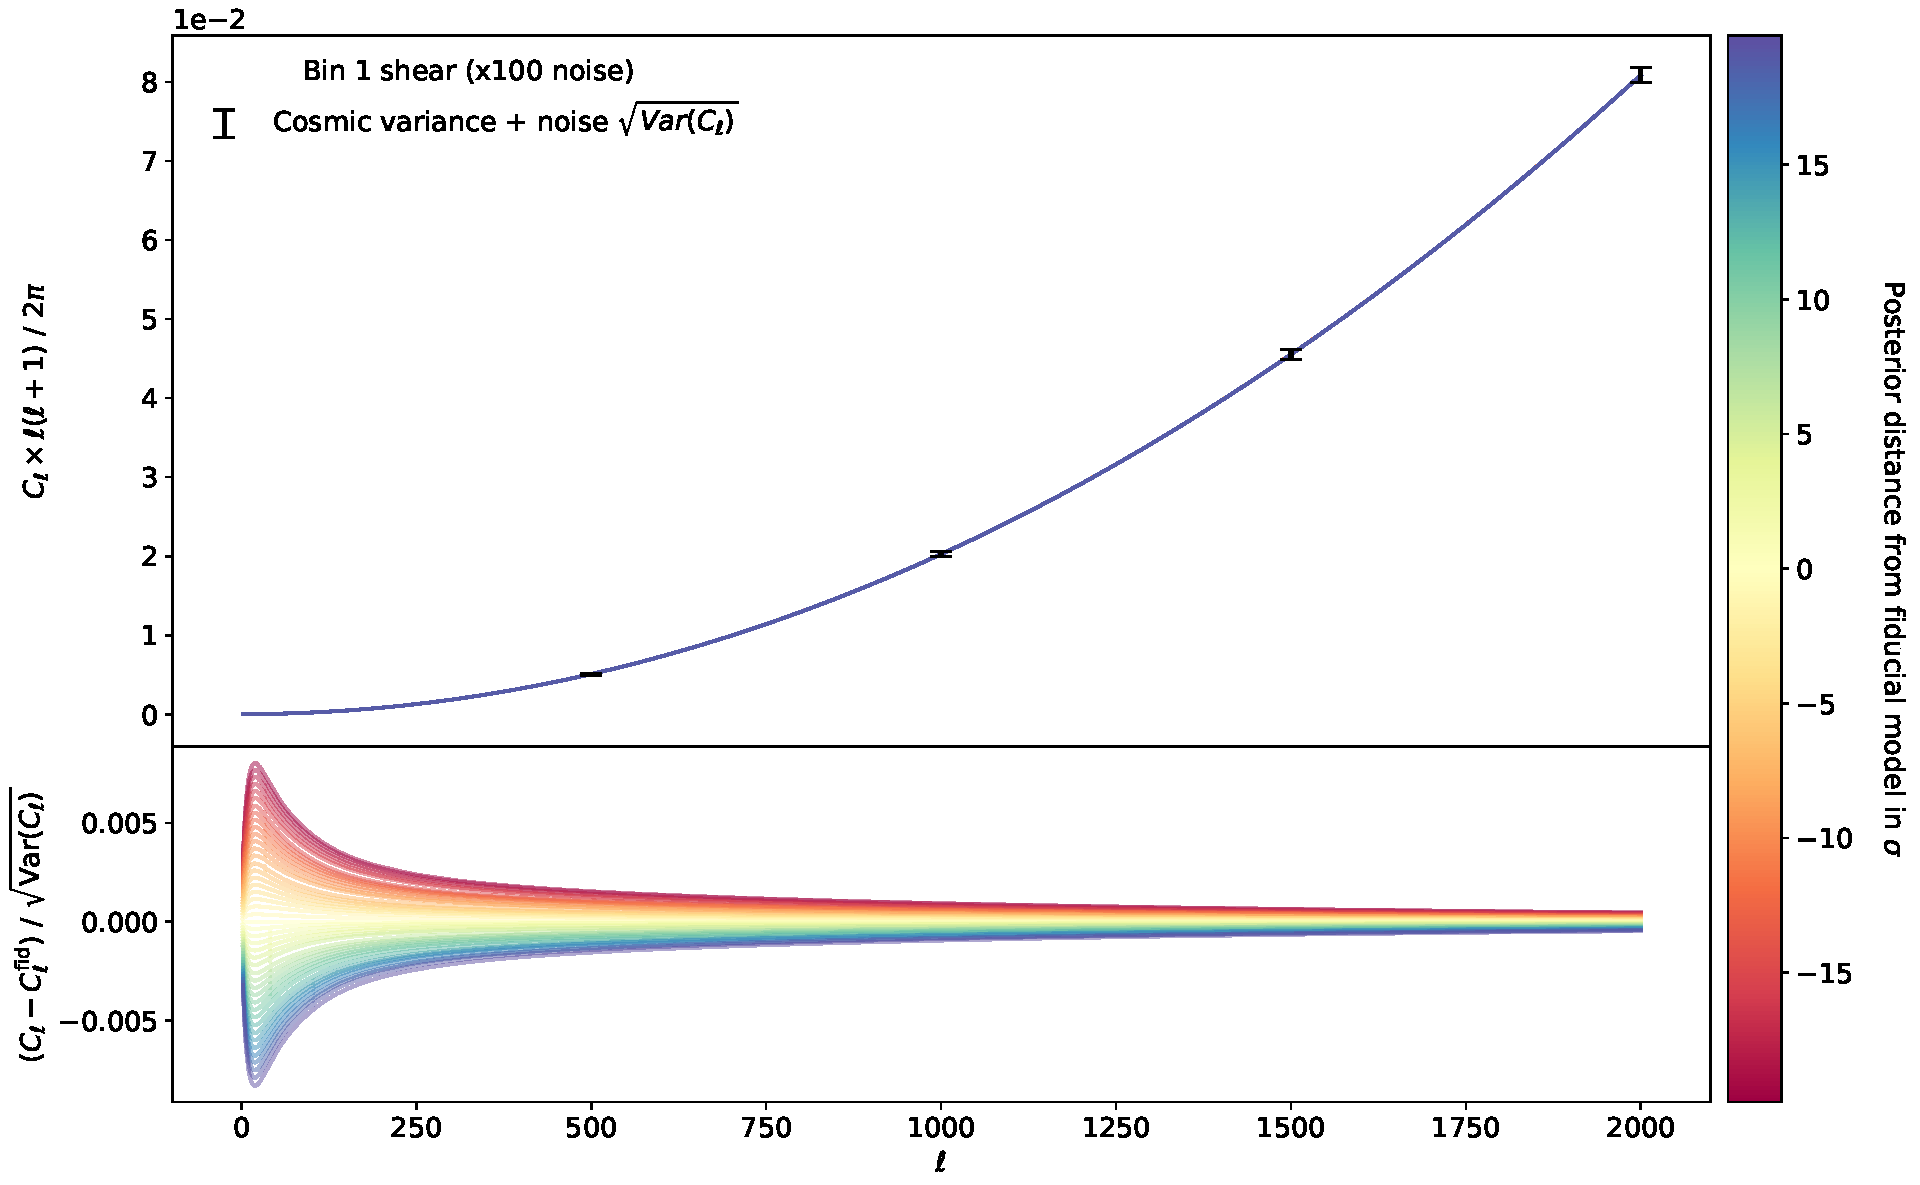
\includegraphics[width=\textwidth]{cl_perl_x100noise}
\caption{As \autoref{bin_Fig:cl_perl} but with 100$\times$ baseline noise. Top: 45 theoretical power spectra, corresponding to the shear auto-power in the lowest redshift bin for different points in the $\wo$--$\wa$ plane. The points are chosen from a diagonal line running perpendicular to the $\wo$--$\wa$ degeneracy direction. Each model is coloured by its distance in $\sigma$ from the fiducial model, determined from a full-sky unbinned power spectrum likelihood analysis. In practice, the 45 power spectra all appear on top of one another. Error bars are shown at a selection of multipoles, and include a shape noise contribution. Bottom: The difference between each model and the fiducial model, scaled by the error bar for each $\ell$.}
\label{bin_Fig:cl_perl_x100noise}
\end{figure}

\begin{figure}[tp]
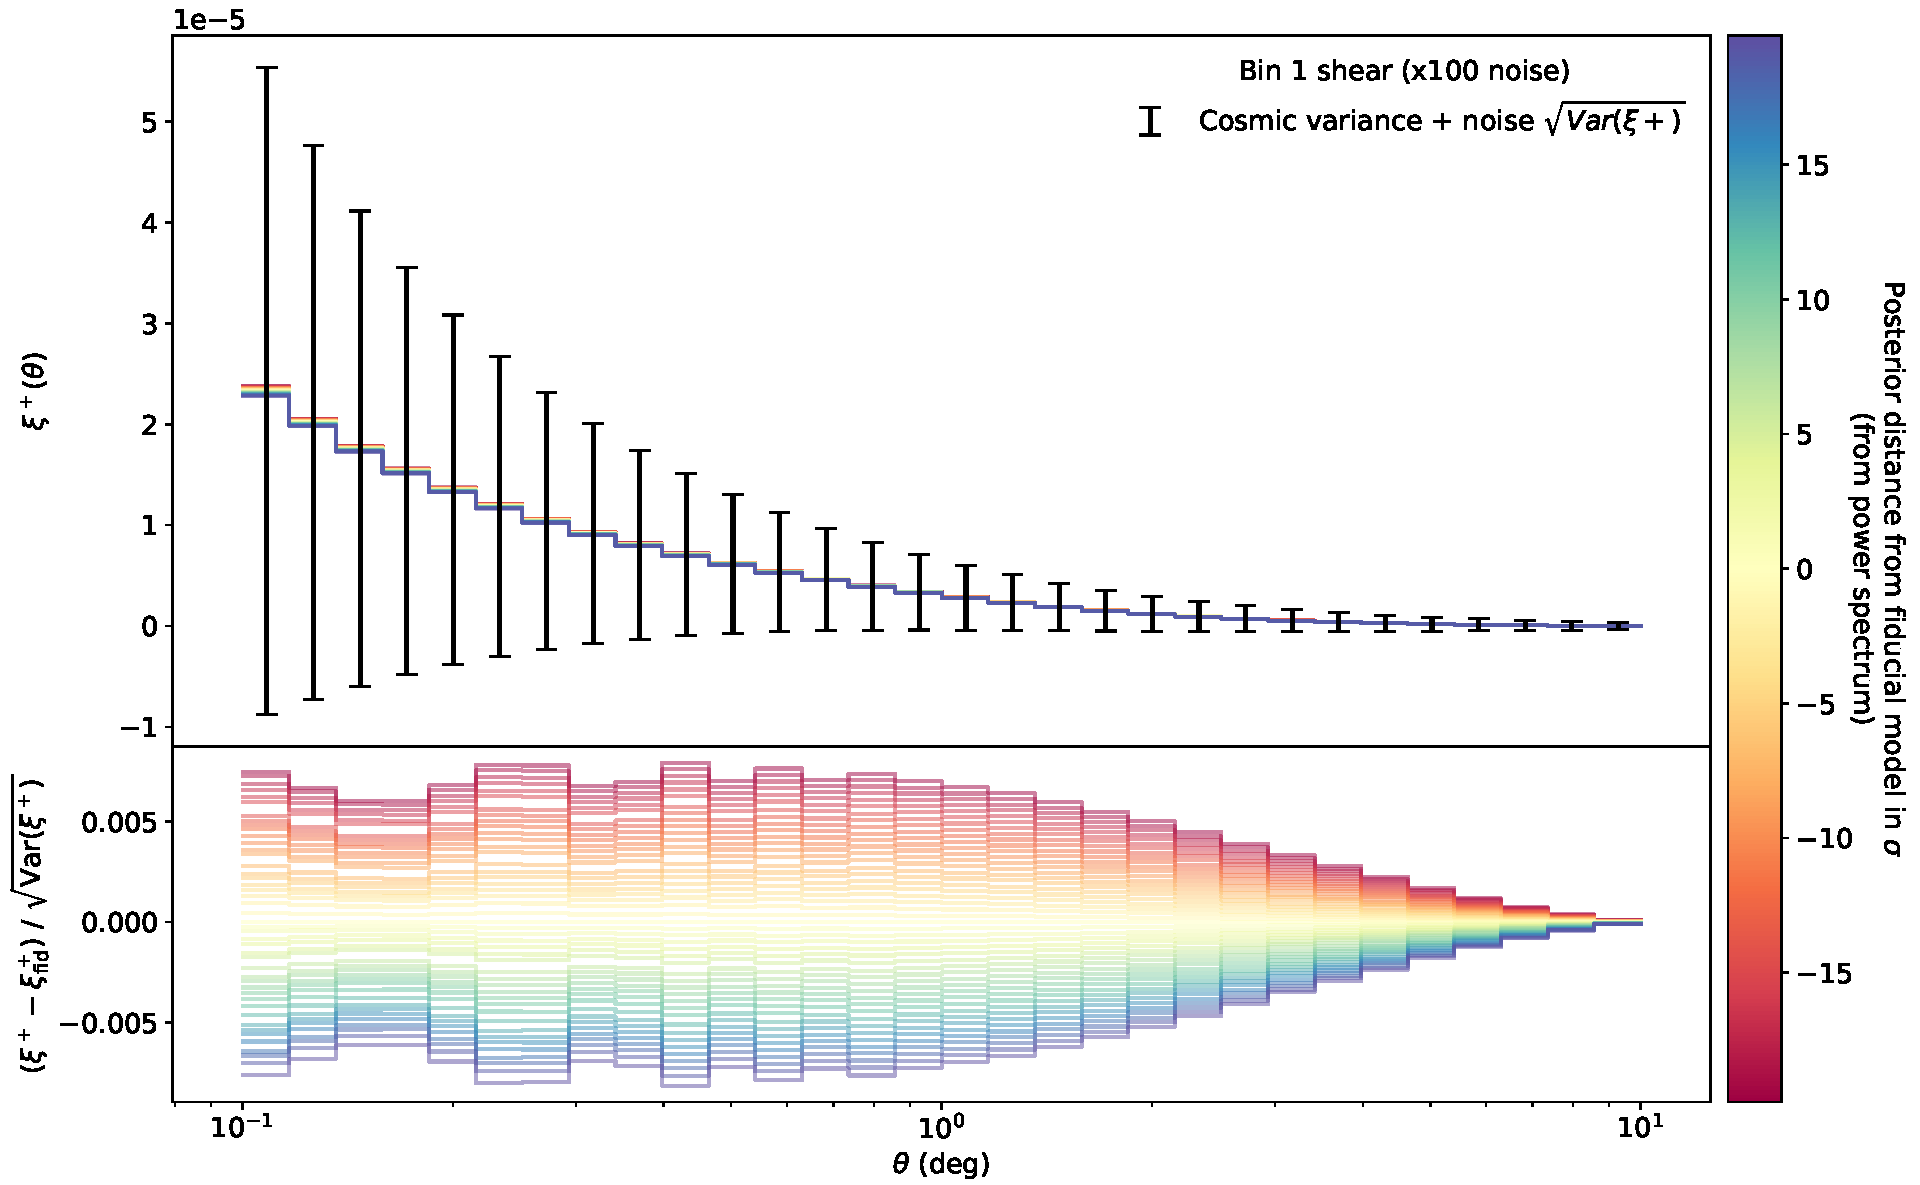
\includegraphics[width=\textwidth]{cf_perbin_x100noise}
\caption{As \autoref{bin_Fig:cf_perbin} but with 100$\times$ baseline noise. Top: 45 theoretical correlation functions, corresponding to $\xi^+$ in the lowest redshift bin for different points in the $\wo$--$\wa$ plane. The points are chosen from a diagonal line running perpendicular to the $\wo$--$\wa$ degeneracy direction. Each model is coloured by its distance in $\sigma$ from the fiducial model, determined from a full-sky unbinned power spectrum likelihood analysis. Error bars are shown for each angular bin, and include a shape noise contribution. Bottom: The difference between each model and the fiducial model, scaled by the error bar for each angular bin.}
\label{bin_Fig:cf_perbin_x100noise}
\end{figure}

\autoref{bin_Fig:cf_perbin_x100noise} shows the equivalent for the correlation function. Compared to the baseline noise level seen previously in \autoref{bin_Fig:cf_perbin}, there is little change in shape when the noise is increased. This is unlike the power spectrum, and explains why the dependence on the number of correlation function bins sees little change when the noise level is varied.

\section{Conclusions}
\label{bin_sec:conclusions}

This chapter has investigated the question of how the statistical uncertainties in the posterior distributions of cosmological parameters derived from weak lensing two-point statistics depend on the number of angular bins used in the analysis. In \autoref{bin_sec:main_analysis} it was shown that for some parameters such as $\wo$ and $\wa$, these uncertainties for the power spectrum only increase by 7--20 per cent even for a single bandpower, relative to 30 bandpowers. In contrast, for the correlation function there is a sharp divergence by several hundred per cent at around 5 angular bins. However, these results vary quite substantially depending on the parameters in question and other aspects of the analysis. For example, power spectrum constraints in $\omb$ and $h$ can degrade by over 200 per cent for low numbers of bandpowers, while the same parameters do not suffer quite as badly for the correlation function. There is an inconsistent dependence on scale cut: a selection of four cosmological parameters ($\wo$, $\wa$, $\omm$, $\sie$) exhibit a dependence of $\sqrt{\lmax}$ for the power spectrum, but not for the correlation function, while the other parameters investigated ($\omb$, $h$, $n_s$) show no such dependence.

In \autoref{bin_sec:additional_effects} a number of additional effects have been investigated. It was shown in \autoref{bin_sec:fsky} that the use of the `$\fsky$ approximation' for the power spectrum covariance leads to similar results to using the full Improved NKA method. The different behaviour of the power spectrum and correlation function for small numbers of bins was investigated in \autoref{bin_sec:low_nbin}, where it was shown that this arises from the different ways in which scales are weighted within each angular bin. Finally, the effect of noise was studied in \autoref{bin_Sec:noise}, where it was shown that the number of angular bins needed for the correlation function has no strong dependence on the level of noise, but that a higher noise level in the power spectrum requires more bandpowers.

While there is no single rule for the number of required angular bins that captures all possible analysis setups, the results in this chapter suggest that, for instance, if a maximum degradation on parameter uncertainties of 10 per cent is required, then 10 bandpowers appears comfortably sufficient for power spectra, and 15 angular bins for correlation functions. This is true for any angular range up to at least $\lmax = 5000$ ($\tmin = 0.03\,\text{deg}$), although significantly higher scale cuts than this may require more bins.


% % Uncomment to build alone without subfiles:
% \emergencystretch=.4em % to avoid overfull hboxes
% \printbibliography[heading=bibintoc]
% \end{document}
